% !TeX spellcheck = it_IT
% !TXS template
\documentclass[italian]{article}
\usepackage[T1]{fontenc}
\usepackage[utf8]{inputenc}
\usepackage{lmodern}
\usepackage[a4paper,top=3cm,bottom=3cm,left=2.5cm,right=2.5cm]{geometry}
\usepackage[italian]{babel}
\usepackage{enumitem}
\usepackage[fleqn]{amsmath}
\usepackage{amssymb}
\usepackage{mathtools}% http://ctan.org/pkg/mathtools
\usepackage{cancel}
\usepackage{color}
\usepackage[usenames,dvipsnames]{xcolor}
\usepackage{units}
\usepackage{hyperref}
\usepackage{textcomp}
\usepackage{soul}
\usepackage{listings}
\usepackage{pifont} %https://www.rpi.edu/dept/arc/training/latex/LaTeX_symbols.pdf
\usepackage{fontspec}
\usepackage{fontawesome}
\usepackage{mdframed}
\usepackage{pgf,tikz}
\usepackage{mathrsfs}
\usetikzlibrary{arrows}
\usepackage{multicol}
\usepackage{titlesec}
\usepackage{amsthm}

\hypersetup{
	colorlinks,
	citecolor=black,
	filecolor=black,
	linkcolor=black,
	urlcolor=blue
}

% SubSubSubSection
%\titleclass{\subsubsubsection}{straight}[\subsection]
%\newcounter{subsubsubsection}[subsubsection]
%\renewcommand\thesubsubsubsection{\thesubsubsection.\arabic{subsubsubsection}}
%\renewcommand\theparagraph{\thesubsubsubsection.\arabic{paragraph}} % optional; useful if paragraphs are to be numbered
%\titleformat{\subsubsubsection}
%{\normalfont\normalsize\bfseries}{\thesubsubsubsection}{1em}{}
%\titlespacing*{\subsubsubsection}
%{0pt}{3.25ex plus 1ex minus .2ex}{1.5ex plus .2ex}

%\makeatletter
%\renewcommand\paragraph{\@startsection{paragraph}{5}{\z@}%
%	{3.25ex \@plus1ex \@minus.2ex}%
%	{-1em}%
%	{\normalfont\normalsize\bfseries}}
%\renewcommand\subparagraph{\@startsection{subparagraph}{6}{\parindent}%
%	{3.25ex \@plus1ex \@minus .2ex}%
%	{-1em}%
%	{\normalfont\normalsize\bfseries}}
%\def\toclevel@subsubsubsection{4}
%\def\toclevel@paragraph{5}
%\def\toclevel@paragraph{6}
%\def\l@subsubsubsection{\@dottedtocline{4}{7em}{4em}}
%\def\l@paragraph{\@dottedtocline{5}{10em}{5em}}
%\def\l@subparagraph{\@dottedtocline{6}{14em}{6em}}
%\makeatother
%\setcounter{secnumdepth}{4}
%\setcounter{tocdepth}{4}
% End SubSubSubSection

\renewcommand{\labelitemii}{$\circ$}
\newcommand{\powerset}[1]{\mathcal{P}(#1)}

\newcommand{\linea}{\begin{center}\rule{5cm}{1pt}\end{center}}
\newcommand{\crossmark}{\textcolor{red}{\text{\ding{56}}}}
\renewcommand{\checkmark}{\textcolor{ForestGreen}{\text{\ding{52}}}}
\newcommand{\ins}[1]{\text{$\mathbb{#1}$}}
\newcommand{\dateright}[1]{\normalfont{\normalsize{\hfill #1 \\}}}
\renewcommand{\dim}[1]{\text{dim$\left(#1\right)$}}
\newcommand{\taleche}{\;|\;}
\newcommand{\len}[1]{\text{$|#1|$}}
\newtheorem*{theorem*}{Teorema}
\newtheorem*{definition*}{Definizione}
\newtheorem*{corollary*}{Corollario}
\newtheorem*{lemma*}{Lemma}
\newtheorem*{exercize*}{Esercizio}

\let\oldexists\exists
\renewcommand{\exists}{\text{$\;\oldexists$}}

\let\oldsharp\sharp
\renewcommand{\sharp}{\text{$\#$}}

\newcommand{\homeExercize}{\text{\faHome $\;$ Esercizio per casa}}
\newcommand{\example}{\noindent\textbf{Esempio.\quad}}
\newcommand{\derive}{\overset{*}{\Rightarrow}}
\newcommand{\To}{\Rightarrow}


\definecolor{ao(english)}{rgb}{0.0, 0.5, 0.0}

\lstset{language=C,
	basicstyle=\ttfamily,
	keywordstyle=\color{blue}\ttfamily,
	stringstyle=\color{red}\ttfamily,
	commentstyle=\color{ao(english)}\ttfamily,
	morecomment=[l][\color{magenta}]{\#}
}

\author{Giacomo De Liberali}

\begin{document}
	
\title{Calcolabilità e Linguaggi Formali}
\maketitle

\tableofcontents
\pagebreak

\section{Introduzione}
\dateright{21 Settembre 2017}
Gli argomenti trattati in questo corso sono:

\begin{enumerate}
	\item Teoria degli automi (capitoli $1,2,3$)
	\item Calcolabilità: cosa si può computare? (capitili $3,4,5$) 
	\item Complessità delle soluzioni
\end{enumerate}

\section{Linguaggi regolari}
Il modello di computazione più elementare sono gli automi a stati finiti. Andiamo a rappresentare tramite un automa una porta con una bilancia da ogni lato che permetta l'accesso alle persone e impedisca alla porta stessa di colpire qualcuno:

\begin{center}
	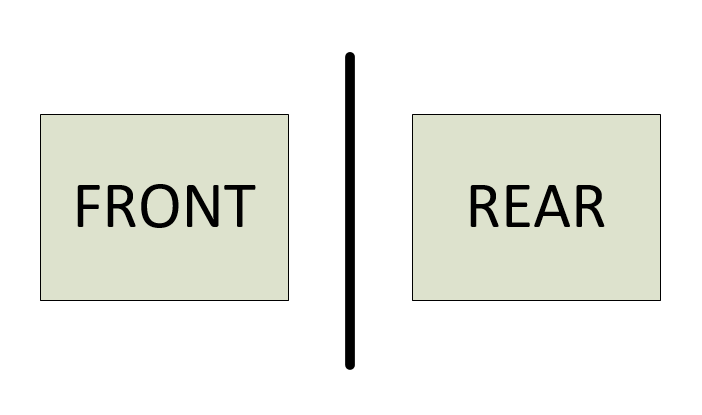
\includegraphics[width=0.3\linewidth]{images/door}
\end{center}
La pressione della pedana \textit{Font} comporterà quindi l'apertura della porta. I possibili input sono quattro:
\begin{enumerate}
	\item Front
	\item Rear
	\item Both
	\item Neither
\end{enumerate}

e rappresentati in un automa:

\begin{center}
	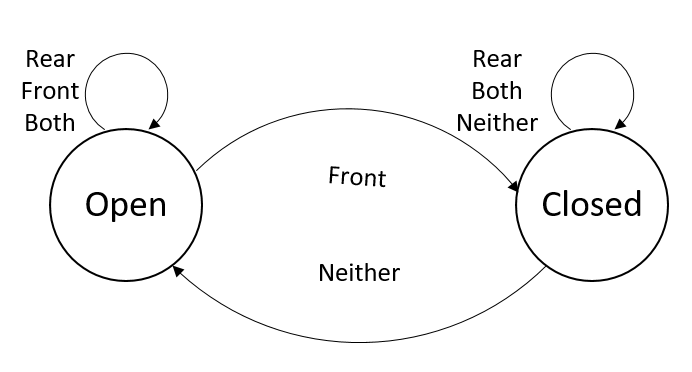
\includegraphics[width=0.5\linewidth]{images/automa1}
\end{center}

\pagebreak

\section{Automa a stati finiti}
\subsection{Definizione}
\label{sec:automDefinition}
Un automa a stati finiti è una 5-tupla $(Q,\;\Sigma,\;\delta,\;q_0,\;F)$ dove:
\begin{enumerate}
	\item $Q$ è un insieme finito di stati
	\item $\Sigma$ è un insieme finito di simboli (detto \textit{alfabeto})
	\item $\delta$ è la \textit{funzione di transizione} che data una coppia stato-alfabeto ritorna uno stato: $\delta: Q\times\Sigma \to Q$
	\item $q_0 \in Q$ è lo stato iniziale (negli automi è ammesso solo \underline{uno} stato iniziale)
	\item $F \subseteq Q$ è un insieme degli stati finali (o \textit{accettanti})
\end{enumerate}
\example
\begin{center}
	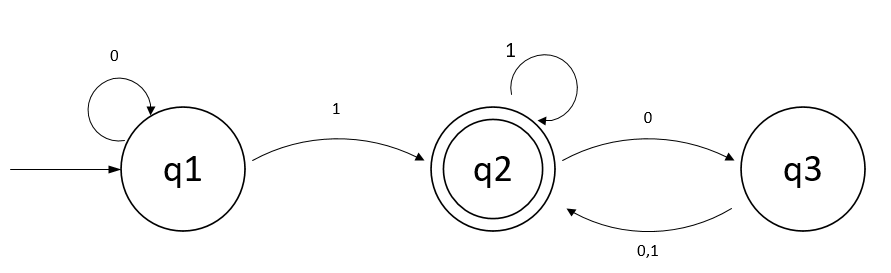
\includegraphics[width=0.8\linewidth]{images/automa2}
\end{center}
L'automa può essere rappresentato formalmente mediante la seguente sintassi:
\[
	A = (\{q_1,q_2,q_3\},\; \{0,1\},\; \delta,\; q_1,\; \{q_2\}) 
\]
dove $\delta$ è definita come:
\begin{gather*}
	\delta(q_1,0) = q_1 \qquad \delta(q_1,1) = q_2 \\
	\delta(q_2,0) = q_3 \qquad \delta(q_2,1) = q_2 \\
	\delta(q_3,0) = q_2 \qquad \delta(q_3,1) = q_2
\end{gather*}
Analizzando le stringhe che l'automa accetta, possiamo notare che quelle valide (e quindi accettate) sono tutte quelle che
\begin{enumerate}
	\item finiscono con $1$
	\item oppure finiscono con $0$ e hanno un numero pari di $0$ dopo l'ultimo $1$
\end{enumerate}
Ad esempio, la stringa $1101$ è una stringa valida in quanto alla fine dell'input l'automa è nello stato $q_2$ che è l'unico stato finale.
\pagebreak \\
\example
\begin{center}
	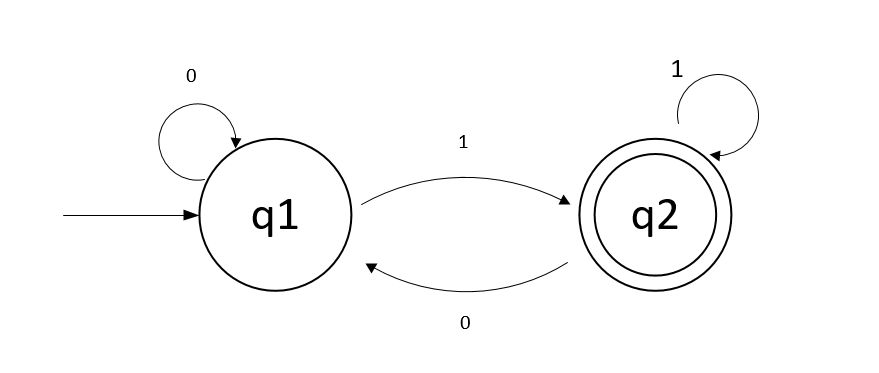
\includegraphics[width=0.5\linewidth]{images/automa3}
\end{center}
Questo automa riconosce stringhe in $\{0,1\}$ che finiscono per $1$. Nel caso di stringa vuota ($\varepsilon$) non entro in nessuno stato e non mi muovo. \\\\
\example
\begin{center}
	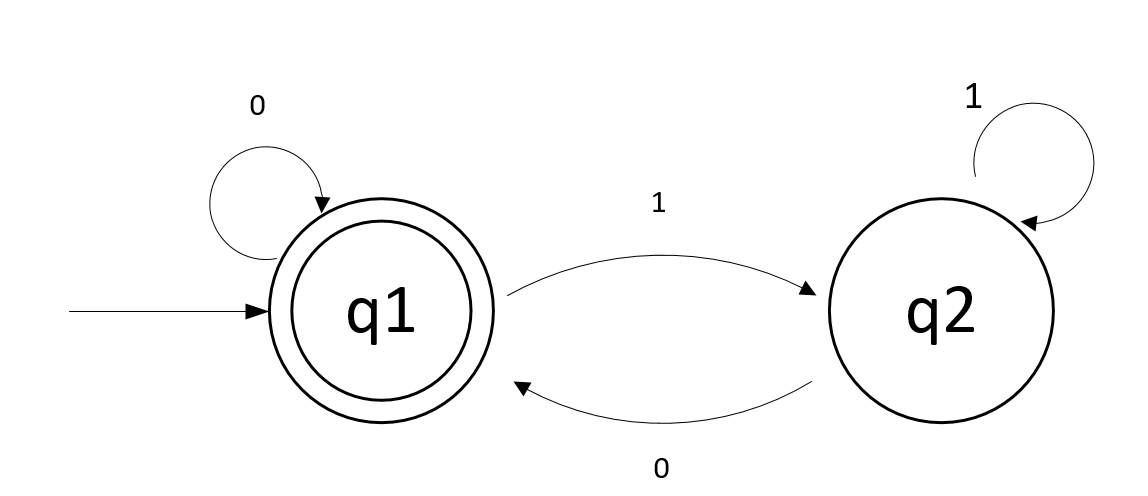
\includegraphics[width=0.5\linewidth]{images/automa4}
\end{center}
Questo automa riconosce stringhe in $\{0,1\}$ che finiscono per $0$ oppure $\varepsilon$.\\\\
\example
\begin{center}
	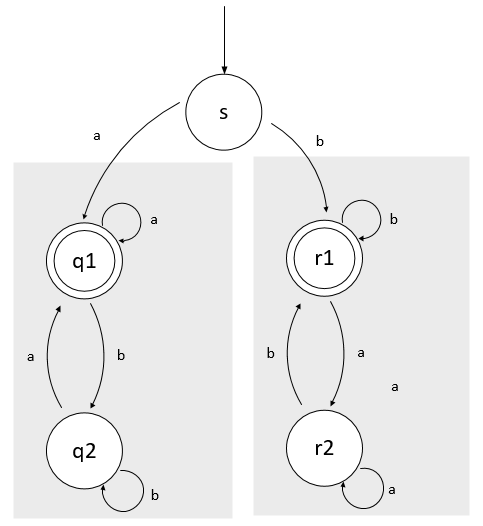
\includegraphics[width=0.5\linewidth]{images/automa5}
\end{center}
Questo automa riconosce stringhe in $\{a,b\}$ che iniziano e finiscono per lo stesso simbolo. In automi come in questo caso è utile poter scomporre il problema in più sotto-problemi Possiamo notare infatti che una volta scelto uno dei due rami che non è possibile passare all'altro. Questo suggerisce di studiare singolarmente i due automi sinistro e destro e infine di comporre la soluzione. \\\\
L'automa di sinistra accetta stringhe che iniziano e finiscono solo per $a$, mentre l'automa di sinistra solo stringhe che iniziano e finiscono per $b$.\\\\
\example
\begin{center}
	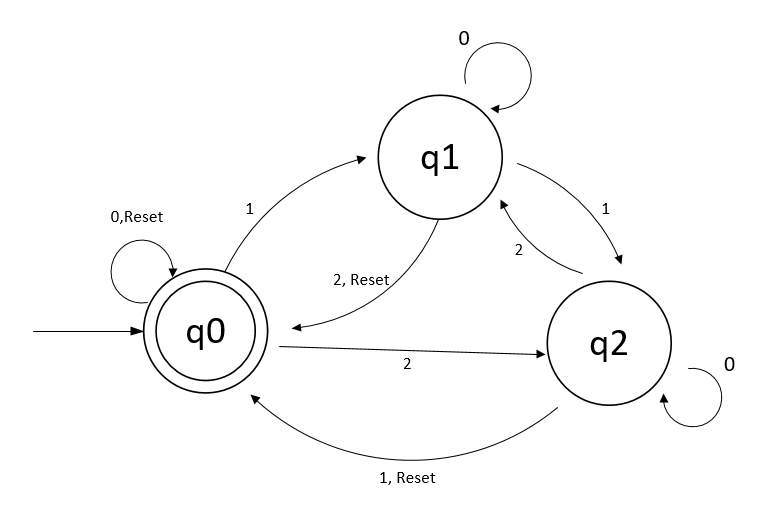
\includegraphics[width=0.5\linewidth]{images/automa6}
\end{center}
Questo automa fa la somma modulo $3$ di tutti i numeri letti in input dopo l'ultimo simbolo di \textit{Reset}, se esiste. 

\subsection{Accettazione di una stringa}
Sia $M = (Q,\;\Sigma,\;\delta,\;q_0,\;F)$ un automa a stati finiti e sia $w = w_1, ..., w_n$ una stringa tale che 
\[
	\forall i \in [1...n] : w_i \in \Sigma
\]
Diciamo che $M$ accetta $w$ se e solo se esiste una sequenza di stati $R_0,R_1,...,R_n \in Q$ tali che
\begin{enumerate}
	\item $R_0 = q_0$ (partendo dal nodo iniziale)
	\item $R_n \in F$ (terminando in uno stato finale)
	\item $\forall i \in [0,n-1] : \sigma(R_i,w_{i+1}) = R_{i+1}$ (per ogni input la \hyperref[sec:automDefinition]{\underline{\textit{funzione di transizione}}} termini in uno stato finale)
\end{enumerate}
$M$ riconosce il linguaggio $A$ se e solo se
\[
	A = \{ w \taleche M \text{ accetta } w \}
\]
Un linguaggio $A$ è \textit{regolare} se e solo se esiste un automa a stati finiti $M$ tale che $M$ riconosce $A$. \\
\pagebreak \\
\example: alfabeto $\{0,1\}$ e vogliamo riconoscere tutte le stringhe con un numero dispari di $1$. L'idea è di avere un bit di informazione, quindi due stati, che mi rappresentano la condizione: ho contanto un numero pari di $1$ oppure ho contanto un numero dispari di $1$. L'automa è il seguente:
\begin{center}
	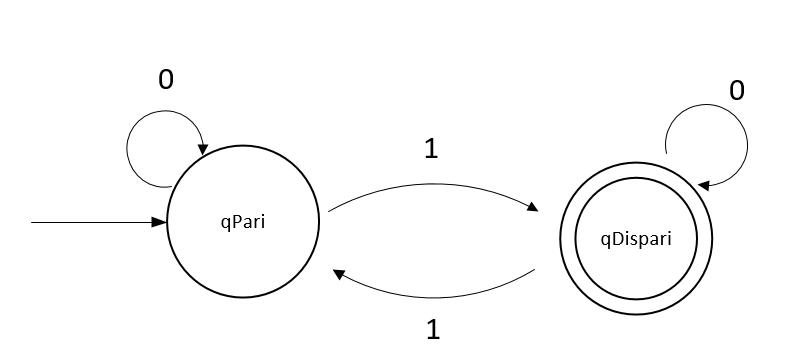
\includegraphics[width=0.5\linewidth]{images/automa7}
\end{center}
\example: alfabeto $\{0,1\}$ e vogliamo riconoscere tutte le stringhe che contengono almeno una volta la sotto-stringa $001$. L'invariante è:
\begin{enumerate}
	\item $q_0$: non ho letto sequenze di $001$
	\item $q_1$: ho letto $0$
	\item $q_2$: ho letto $00$
	\item $q_3$: ho letto $001$
\end{enumerate}
\begin{center}
	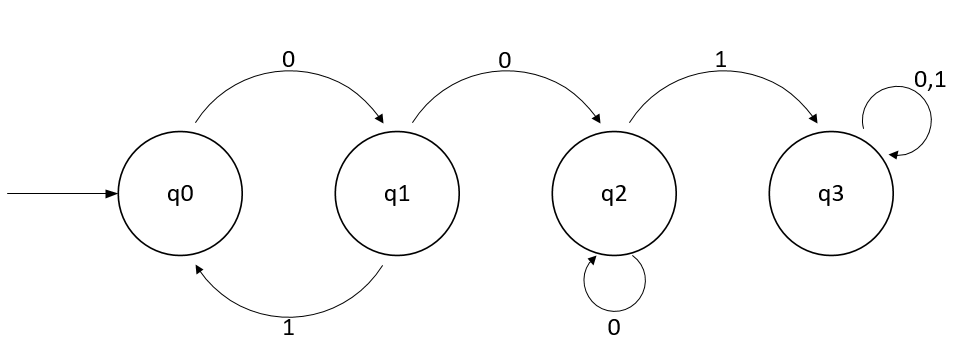
\includegraphics[width=0.6\linewidth]{images/automa8}
\end{center}
\pagebreak
\subsection{Operazioni regolari}
Siano $A$ e $B$ due linguaggi. Definiamo le operazioni regolari \textbf{unione}, \textbf{concatenazione} e \textbf{star} come segue:
\begin{enumerate}
	\item \textbf{Unione}: $A \cup B = \{ x \taleche x \in A  \lor x \in B \}$
	\item \textbf{Concatenazione}: $A \circ B = \{ xy \taleche x \in A  \land y \in B \}$
	\item \textbf{Star}: $A^* = \{ x_1x_2\dots x_n \taleche k \geq 0 \land \forall i \; x_i \in A \}$
\end{enumerate} 
L'operazione \textit{star} è un'operazione unaria e non binaria come le altre due. Si applica quindi ad un solo linguaggio invece che a due. Funziona combinando le stringhe in $A$ con se stesse per ottenere una stringa nel nuovo linguaggio. Poiché ogni numero include $0$ come possibilità, la stringa vuota $\varepsilon$ è sempre un membro di $A^*$, indipendentemente da cosa $A$ sia.\\\\
\example: sia $\Sigma$ l'alfabeto composto dalle $26$ lettere standard $\{ a,b,\dots,z \}$. Se $A = \{ \text{good},\text{bad} \}$ e $B = \{ \text{boy},\text{girl} \}$ allora:
\begin{itemize}[label={}]
	\item $A \cup B = \{ \text{good},\text{bad}, \text{boy},\text{girl} \}$
	\item $A \circ B = \{ \text{goodboy},\text{goodgirl},\text{badboy}, \text{badgirl} \}$
	\item $A^* = \{ \varepsilon, \text{good},\text{bad},\text{goodgood}, \text{goodbad}, \text{badgood}, \\ \text{badbad}, \text{goodgoodgood}, \text{goodgoodbad}, \text{goodbadgood}, \text{goodbadbad}, \dots \}$
\end{itemize}
Una collezione di oggetti si dice chiusa sotto un'operazione se applicando tale operazione ai membri della collezione l'oggetto ritornato è ancora nella collezione di partenza (es. $\mathbb{N}$ è chiuso rispetto al prodotto ma non rispetto alla divisione).

\subsection{Chiusura}
\subsubsection{Rispetto all'unione}
La classe dei linguaggi regolari è chiusa rispetto all'operazione di unione $\cup$.\\\\
Siano $A_1,A_2$ due linguaggi regolari, vogliamo dimostrare che $A_1 \cup A_2$ è un linguaggio regolare. Poiché $A_1$ e $A_2$ sono regolari, sappiamo che esiste un automa a stati finiti $M_1$ che riconosce $A_1$ ed un automa $M_2$ che riconosce $A_2$. Per dimostrare che $A_1 \cup A_2$ è regolare dimostriamo un automa a stati finiti $M$ che riconosce $A_1 \cup A_2$. \\\\
Sia $M_1 = (Q_1,\Sigma,\delta_1,q_1,F_1)$ e sia $M_2 = (Q_2,\Sigma,\delta_2,q_2,F_2)$, assumendo che abbiano lo stesso alfabeto $\Sigma$, costruiamo $M = (Q,\Sigma,\delta,q,F)$ come segue
\begin{enumerate}
	\item $Q = \{ (r_1,r_2) \taleche r_1 \in Q_1 \land r_2 \in Q_2 \}$. Questo insieme è il prodotto cartesiano degli insiemi $Q_1\times Q_2$. È l'insieme delle coppie degli stati, la prima di $Q_1$ e la seconda di $Q_2$.
	\item $\Sigma$, l'alfabeto, è lo stesso in $M_1$ e $M_2$. Assumiamo per semplicità che sia lo stesso.
	\item $\delta$, la funzione di transizione, è definita come segue. Per ogni $(r_1,r_2) \in Q$ e per ogni $a \in \Sigma$, sia
	\[
		\delta\left( (r_1,r_2),a \right) = \left( \delta_1(r_1,a),\delta_2(r_2,a) \right)
	\]
	Quindi $\delta$ prende uno stato di $M$ (che è una coppia di stati di $M_1$ e $M_2$) insieme ad un simbolo di input e ritorna il prossimo stato di $M$.
	\item $q_0$ è la coppia $(q_1,q_2)$.
	\item $F$ è l'insieme delle coppie nelle quali è accettato lo stato in $M_1$ oppure $M_2$. Possiamo scriverla come
	\[
		F = \{ (r_1,r_2) \taleche r_1 \in F_1 \lor r_2 \in F_2 \}
	\]
\end{enumerate}
Questo conclude la costruzione dell'automa $M$ che riconosce l'unione di $A_1$ e $A_2$.
\subsubsection{Rispetto alla concatenazione}
La classe dei linguaggi regolari è chiusa rispetto all'operazione di concatenazione $\circ$.\\\\
Per dimostrare questo teorema dobbiamo anche questa volta costruire un nuovo automa, con la differenza che questa volta non accetterà l'input se lo accetta $M_1$ oppure $M_2$. $M$ deve accettarlo se l'input può essere spezzato in due pezzi, dove $M_1$ accetta il primo pezzo e $M_1$ accetta il secondo pezzo. Il problema è che $M$ non sa quando spezzare l'input. Per risolvere questo problema dobbiamo introdurre il concetto di \textit{non determinismo}.

\subsection{Non determinismo}
Fino ad ora ogni passo di una computazione portava ad un unica via. Quando una macchina è in un dato stato e legge il prossimo simbolo di input, sappiamo quale sarà il prossimo stato. Questo meccanismo viene chiamato \textbf{deterministico}. In un sistema \textbf{non deterministico} scelte differenti possono esistere per il prossimo stato, in ogni punto.
\begin{center}
	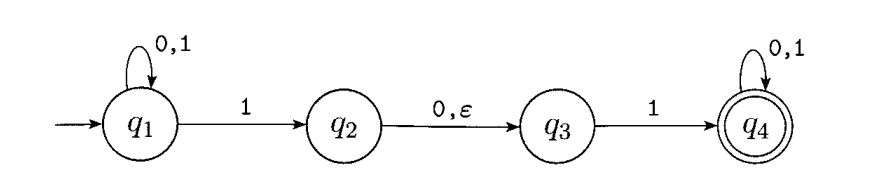
\includegraphics[width=0.5\linewidth]{images/ndautoma1}
\end{center}
La differenza fra un automa a stati finiti deterministico (\textit{DFA}, Deterministic Finite Automaton) e non deterministico  (\textit{NFA}, Nondeterministic Finite Automaton):
\begin{itemize}
	\item Ogni stato di un DFA ha esattamente una freccia uscente per ogni simbolo dell'alfabeto. Un NFA vìola questa regola.
	\item Un stato di un NFA può avere zero, una o più frecce uscenti per ogni simbolo dell'alfabeto (compreso $\varepsilon$).
\end{itemize}
\subsubsection{Come computa un NFA?}
Supponiamo di trovarci in un NFA con una stringa in input che ci ha condotti allo stato $q_1$ che ha più modi di procedere. Per esempio, diciamo che il prossimo simbolo di input è $1$. Dopo aver letto il simbolo la macchina si divide in copie multiple di se stessa e segue \textbf{tutte} le possibili vie in parallelo. Ogni copia della macchina prende una direzione e continua la computazione come prima, dividendosi a sua volta in più copie se necessario. Se il prossimo simbolo di input non compare in nessuna freccia uscente dallo stato corrente di ogni copia, quella copia cessa di esistere assieme al ramo della computazione a lei associato. Alla fine dell'input, se almeno una delle copie si trova in uno stato accettante, il NFA accetta la stringa di input. \\
Se viene incontrato uno stato con una freccia uscente con il simbolo $\varepsilon$, senza nemmeno leggere l'input la macchina se divide in copie multiple, una per ogni freccia uscente marcata da $\varepsilon$ e una copia rimane ferma sullo stato corrente. Successivamente la macchina procede in modo non deterministico come prima.
\begin{center}
	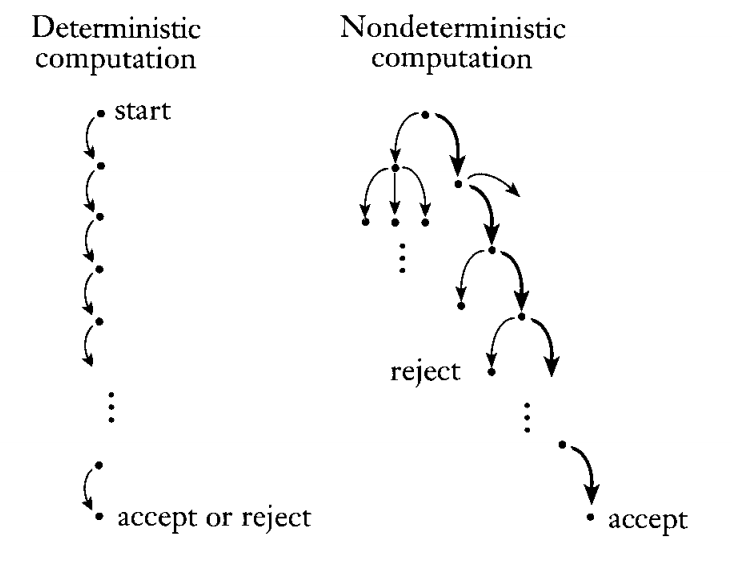
\includegraphics[width=0.5\linewidth]{images/nondeterministic}
\end{center}
\example di computazione non deterministica dell'automa visto sopra con l'input $010110$:
\begin{center}
	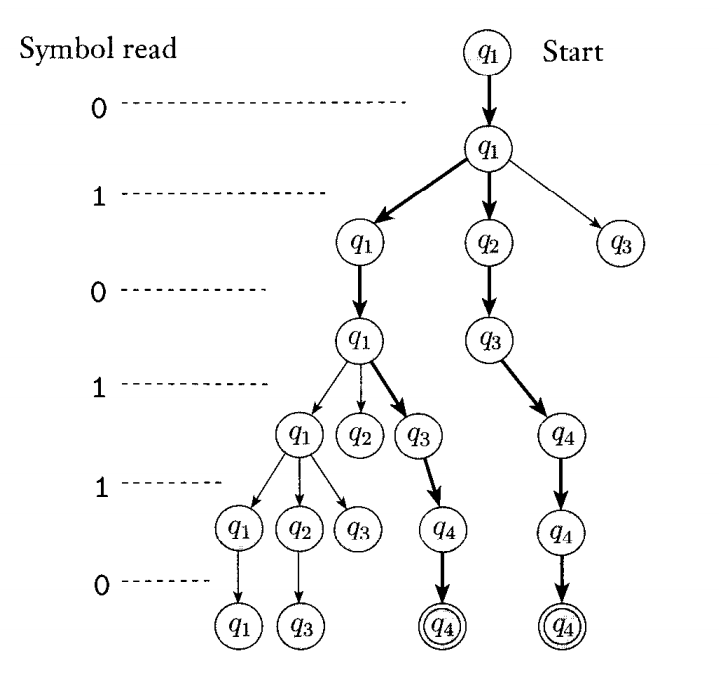
\includegraphics[width=0.7\linewidth]{images/branches}
\end{center}
\example: sia $A$ il linguaggio che consiste in tutte le stringhe in $\{0,1\}$ che contengono un $1$ nella terza posizione dalla fine (es. $000100$). Il seguente NFA a tre stati riconosce $A$:
\begin{center}
	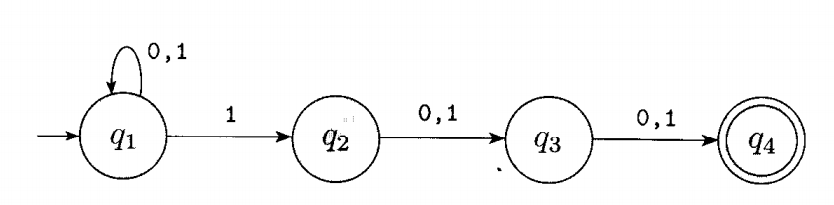
\includegraphics[width=0.5\linewidth]{images/nfa_1}
\end{center}
\pagebreak
\subsubsection{Definizione}
Una NFA è una quantupla $(Q,\;\Sigma,\;\delta,\;q_0,\;F)$ dove:
\begin{enumerate}
	\item $Q$ è un insieme finito di stati
	\item $\Sigma$ è un insieme finito di simboli detto alfabeto
	\item $\delta: Q\times (\Sigma \cup \{\varepsilon\}) \to \powerset{Q}$ 
	\item $q_0 \in Q$ è lo stato iniziale 
	\item $F \subseteq Q$ è un insieme degli stati finali 
\end{enumerate}
\example
\begin{center}
	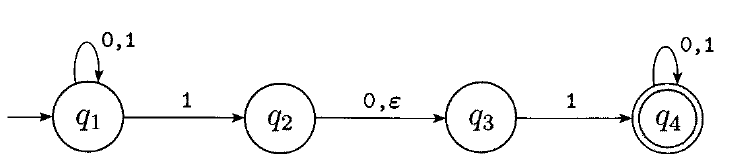
\includegraphics[width=0.7\linewidth]{images/nfa_2}
\end{center}
L'automa può essere rappresentato formalmente mediante la seguente sintassi:
\[
	A = (\{q_1,q_2,q_3,q_4\},\; \{0,1\},\; \delta,\; q_1,\; \{q_4\}) 
\]
dove $\delta$ è definita come:
\begin{table}[h!]
	\begin{tabular}{@{}llll}
			$\delta(q_1,0) = \{q_1\}$ & $\delta(q_2,0) = \{q_3\}$ & $\delta(q_3,0) = \varnothing$ & $\delta(q_4,0) = \{q_4\}$\\
			$\delta(q_1,1) = \{q_1,q_2\}$ & $\delta(q_2,1) = \varnothing$ & $\delta(q_3,1) = \{q_4\}$ & $\delta(q_4,1) = \{q_4\}$\\
			$\delta(q_1,\varepsilon) = \varnothing$ & $\delta(q_2,\varepsilon) = \{q_3\}$ & $\delta(q_3,\varepsilon) = \varnothing$ & $\delta(q_4,\varepsilon) = \varnothing$
	\end{tabular}
\end{table}
\subsubsection{Accettazione di una stringa}
Sia $N = (Q,\;\Sigma,\;\delta,\;q_0,\;F)$ un NFA. Diciamo che $N$ accetta una stringa $w$ nell alfabeto $\Sigma$ se e solo se $w$ può essere scritta nella forma $y_1,\dots,y_n$ dove $\forall i \in [1,n]:y_i \in \left( \Sigma \cup \{\varepsilon\} \right)$ ed esiste una sequenza di stati $R_0,\dots,R_n \in Q$ tali che:
\begin{itemize}
	\item $R_0$ è lo stato iniziale
	\item $R_m \in F$
	\item $\forall i \in [0,m-1]: R_{i+1} \in \delta(R_i,y_{i+1})$, ovvero che lo stato successivo ($R_{i+1}$) appartiene all'insieme degli stati ottenuti dalla funzione di transizione applicata allo stato corrente ($R_i$) e al prossimo carattere in input ($y_{i+1}$).
\end{itemize}
\subsubsection{Equivalenza tra NFA e DFA}
Dimostrare che ogni NFA ha un equivalente DFA.\\\\
Sia $N = (Q,\;\Sigma,\;\delta,\;q_0,\;F)$ un NFA che riconosce il linguaggio $A$, costruisco un DFA $M = (Q',\;\Sigma,\;\delta',\;q_0',\;F')$ che riconosce esattamente $A$. Assumiamo per semplicità che non vi siano $\varepsilon-$transizioni. Definiamo le componenti di $M$:
\begin{itemize}
	\item $Q' = \powerset{Q}$, insieme delle parti di $Q$
	\item $\delta'(R,a) = \bigcup\limits_{r\in R}\delta(r,a), \quad R \in Q', a \in \Sigma$
	\item $q_0'=\{q_0\}$
	\item $F' = \{R \in \powerset{Q} \;| \exists r \in R, r \in F\}$, ovvero esiste un insieme $R$ nell'insieme delle parti di $Q$ tale che $R$ contenga almeno uno stato accettante (finale) di $N$
\end{itemize}
Verifichiamo che le funzioni di transizione siano ben tipate:
\begin{enumerate}
	\item NFA: $\delta: Q \times \Sigma \to \powerset{Q}$
	\item DFA: $\delta': \underbracket{\powerset{Q}}_{Q'} \times \Sigma \to \underbracket{\powerset{Q}}_{Q'}$
\end{enumerate}
Generalizziamo ora il caso delle $\varepsilon$-transizioni definendo una funzione $E(R) = \{ q \;|\; q \in Q \}$ può essere raggiunto da uno stato in $R$ seguendo solamente $\varepsilon$-transizioni (anche zero). Riformulando i componenti visti sopra:
\begin{itemize}
	\item $\delta'(R,a) =  \bigcup\limits_{r\in R}E\left(\delta(r,a)\right)$
	\item $q_0 = E(\{q_0\})$
\end{itemize}
\subsubsection{Linguaggi regolari}
Andiamo a dimostrare che un linguaggio è regolare se e solo se esiste un NFA che lo riconosce. Dimostrazione:
\begin{itemize}[label={}]
	\item $\Rightarrow$ Se un linguaggio è regolare, per definizione esiste un DFA che lo riconosce. Ma un DFA è un caso speciale di un NFA, quindi la prima parte è dimostrata.
	\item $\Leftarrow$ Sia $A$ un linguaggio tale che $A$ è riconosciuto da un NFA. Per il teorema esiste un DFA che riconosce $A$, quindi $A$ è regolare.
\end{itemize}
\example di conversione di un NFA in un DFA \\\\
NFA:
\begin{center}
	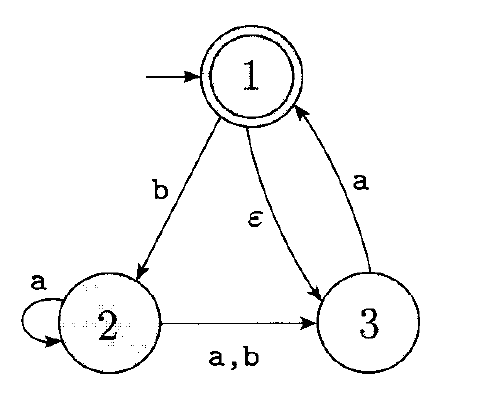
\includegraphics[width=0.3\linewidth]{images/nfa_3}
\end{center}
DFA:
\begin{center}
	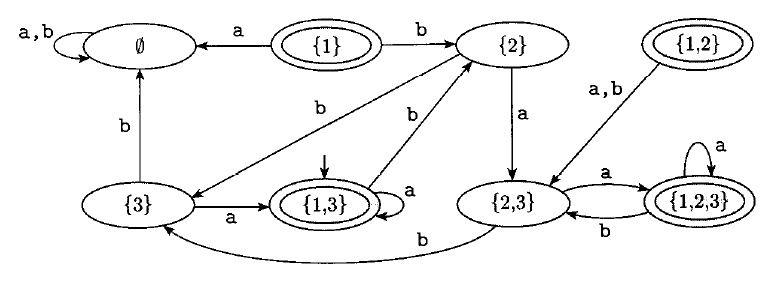
\includegraphics[width=0.7\linewidth]{images/nfa_4}
\end{center}
\paragraph{Chiusura rispetto all'unione}
La classe dei linguaggi regolari è chiusa rispetto all'unione. Dimostrazione: \\\\
Siano $A_1$ e $A_2$ due linguaggi regolari, allora esistono due NFA $N_1$ ed $N_2$ che li riconoscono. Costruisco da $N_1$ ed $N_2$ un NFA che riconosce $A_1\cup A_2$, da cui concludo che $A_1\cup A_2$ è regolare.
\begin{center}
	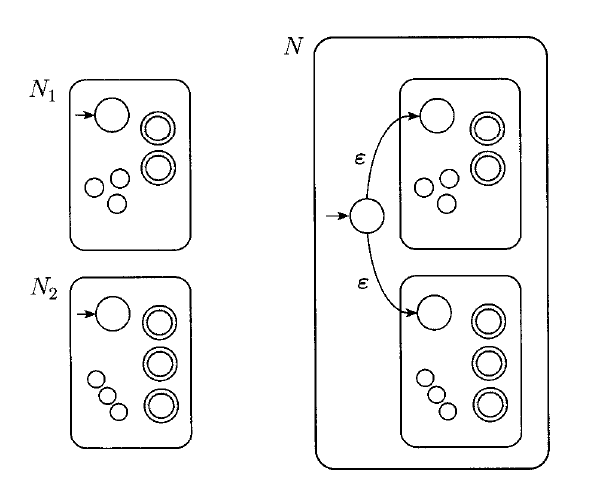
\includegraphics[width=0.7\linewidth]{images/nfa_union}
\end{center}
Definizione formale:
\[
	N_1 = (Q_1,\;\Sigma,\;\delta_1,\;q_1,\;F_1) \qquad N_2 = (Q_2,\;\Sigma,\;\delta_2,\;q_2,\;F_2)
\]
sia 
\[
	O = (Q,\;\Sigma,\;\delta,\;q_0,\;F)
\]
dove:
\begin{itemize}
	\item $Q = Q_1 \cup Q_2 \cup \{q_0\}$
	\item $F = F_1 \cup F_2$
	\item e la funzione di transizione è definita come
		\begin{align*}
		\delta(q,a) = 
		\begin{cases}
			\delta_1(q,a) & \text{se } q \in Q_1 \\
			\delta_2(q,a) & \text{se } q \in Q_2 \\
			\{q_1,q_2\} & \text{se } q=q_0 \land a = \varepsilon \\
			\varnothing & \text{se } q=q_0 \land a \neq \varepsilon 
		\end{cases}
		\end{align*}
\end{itemize}
\pagebreak
\paragraph{Chiusura rispetto alla concatenazione}
La classe dei linguaggi regolari è chiusa rispetto alla concatenazione. Dimostrazione: \\\\
Siano $A_1$ e $A_2$ due linguaggi regolari, allora esistono due NFA $N_1$ ed $N_2$ che li riconoscono.
\begin{center}
	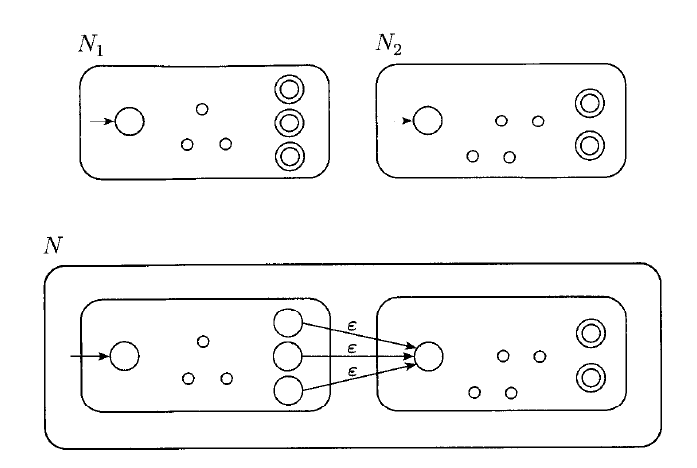
\includegraphics[width=0.7\linewidth]{images/nfa_concat}
\end{center}
In pratica salto dagli stati finali (non più) del primo automa allo stato iniziale del secondo automa. Definizione formale:
\[
	N_1 = (Q_1,\;\Sigma,\;\delta_1,\;q_1,\;F_1) \qquad N_2 = (Q_2,\;\Sigma,\;\delta_2,\;q_2,\;F_2)
\]
sia 
\[
	N = (Q,\;\Sigma,\;\delta,\;q_0,\;F)
\]
dove:
\begin{itemize}
	\item $Q = Q_1 \cup Q_2$
	\item $F = F_2$
	\item e la funzione di transizione è definita come
		\begin{align*}
			\delta(q,a) = 
			\begin{cases}
				\delta_1(q,a) & \text{se } q \in Q_1 \land q \notin F_1 \\
				\delta_1(q,a) & \text{se } q \in F_1 \land a \neq \varepsilon \\
				\delta_1(q,a) \cup \{q_2\} & \text{se } q \in F_1 \land a = \varepsilon\\
				\delta_2(q,a) & \text{se } q \in Q_2 
			\end{cases}
		\end{align*}
\end{itemize}
\pagebreak
\paragraph{Chiusura rispetto all'operazione star}
La classe dei linguaggi regolari è chiusa rispetto all'operazione \textit{star}. Dimostrazione: \\\\
Sia $N_1$ un linguaggio regolare, allora esiste un NFA $N_1$ che lo riconosce. Costruisco un automa $N = (Q,\;\Sigma,\;\delta,\;q_0,\;F)$ che accetta $A^*$:
\begin{center}
	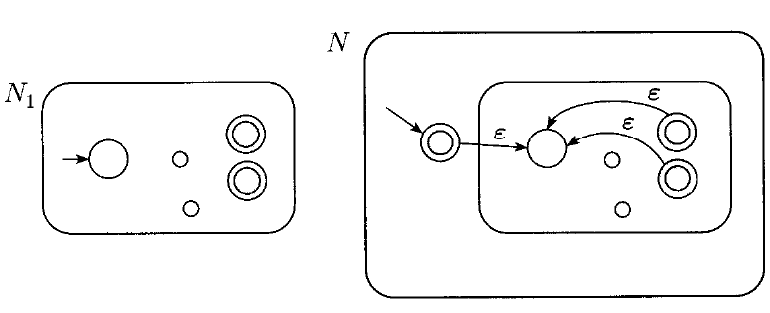
\includegraphics[width=0.7\linewidth]{images/nfa_star}
\end{center}
Aggiungo un primo stato accettante e due $\varepsilon$-transizioni per poter iterare un numero arbitrario di volte. Il primo stato è accettante perche $\varepsilon$ fa sempre parte dei $A^*$. Definizione formale:
\[
	N_1 = (Q_1,\;\Sigma,\;\delta_1,\;q_1,\;F_1)
\]
sia 
\[
	N = (Q,\;\Sigma,\;\delta,\;q_0,\;F)
\]
dove:
\begin{itemize}
	\item $Q = Q_1 \cup \{q_0\}$
	\item $F = \cup \{q_0\}$
	\item e la funzione di transizione è definita come
	\begin{align*}
	\delta(q,a) = 
	\begin{cases}
	\delta_1(q,a) & \text{se } q \in Q_1 \land q \notin F_1 \\
	\delta_1(q,a) & \text{se } q \in F_1 \land a \neq \varepsilon \\
	\delta_1(q,a) \cup \{q_1\} & \text{se } q \in F_1 \land a = \varepsilon\\
	\{\varepsilon\} & \text{se } q = q_0 \land a = \varepsilon \\
	\varnothing & \text{se } q = q_0 \land a \neq \varepsilon
	\end{cases}
	\end{align*}
\end{itemize}
\pagebreak
\section{Espressioni regolari}
Definiamo i linguaggi regolari in modo più compatto e semplice rispetto agli automi:
\[
	L((0\cup 1)0^*) = \{ w \taleche w \text{ inizia con $0$ oppure $1$ e ha un numero arbitrario di $0$}\}
\]
Secondo le regole della precedenza $(^*,\circ,\cup)$, $^*$ è applicabile a $0$ ma non a $(0\cup 1)$.
\subsection{Definizione}
Diciamo che $R$ è un espressione regolare su un alfabeto $\Sigma$ se $R$ è:
\begin{enumerate}
	\item $a \taleche a \in \Sigma$, ovvero se è un membro dell'alfabeto (che è sempre un'espressione regolare) \hfill $L(a) = \{a\}$
	\item $\varepsilon$ \hfill $L(\varepsilon) = \{\varepsilon\}$
	\item $\varnothing$ \hfill $L(\varnothing) = \{\varnothing\}$
	\item $(R_1 \cup R_2)$, dove $R_1$ e $R_2$ sono espressioni regolari \hfill $L((\overbracket{R_1}^{\mathclap{\text{regexp}}} \cup R_2)) = \overbracket{L(R_1)}^{\mathclap{\text{linguaggio regolare}}} \cup L(R_2)$
	\item $(R_1 \circ R_2)$, dove $R_1$ e $R_2$ sono espressioni regolari  \hfill $L((R_1 \circ R_2)) = L(R_1) \circ L(R_2)$
	\item $(R_1^*)$, dove $R_1$ è un'espressione regolare \hfill $L(R_1^*) = L(R_1)^*$
\end{enumerate}
\example in $\Sigma = \{0,1\}$:
\begin{itemize}
	\item $L(0^*10^*) = \{ w \taleche w \text{ contiene esattamente un 1} \}$
	\item $L(01\cup 10) = \{ 01,10 \}$
	\item $L((0\cup \varepsilon)1^*) = \{ w \taleche w \text{ è una stringa di soli $1$ possibilmente preceduta da $0$ } \}$
	\item $L(1^* \circ \varnothing) = \varnothing$, concatenando l'insieme vuoto con qualunque altra cosa si ottiene insieme vuoto
	\item $L(\varnothing^*) = \{\varepsilon\}$, l'operatore di star su un insieme vuoto ritorna la combinazione di $0$ stringhe, ovvero solamente stringa vuota
\end{itemize}
Identità delle espressioni regolari, dove $R$ è una \textit{regexp}:
\begin{itemize}
	\item $R \cup \varnothing = R \quad \checkmark$
	\item $R \cup \varepsilon = R \quad \crossmark$
	\item $R \circ \varepsilon = R \quad \checkmark$
	\item $R \circ \varnothing = R \quad \crossmark$
\end{itemize}
\pagebreak
\subsection{Equivalenza con automi a stati finiti}
\begin{theorem*}
Un linguaggio è regolare se e solo se esiste un'espressione regolare che lo descrive. Quindi $A$ è regolare se e solo se esiste una \textit{regexp} in $R$ tale che $L(R) = A$.
\end{theorem*}
\noindent
Essendo un \textit{se e solo se} vanno dimostrate entrambe le parti.
\begin{lemma*}
	Se $A$ è descritto da una rgexp, allora $A$ è regolare.
\end{lemma*}
\noindent Sia $A$ descritto da una regexp $R$. Per induzione sulla struttura di $R$ procediamo per casi:
\begin{enumerate}[label=\arabic*)]
	\item $R = a$ per qualche $a \in \Sigma$, Dimostro che $L(a)$ è regolare se trovo un NFA che lo riconosca:
	\begin{center}
		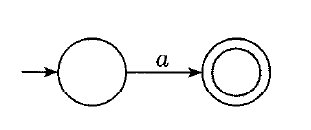
\includegraphics[width=0.3\linewidth]{images/regexp_dim_1}
	\end{center}
	%
	\item $R = \varepsilon$. Allora $L(R) = \{ \varepsilon \}$, e il seguente NFA riconosce $L(R)$
	\begin{center}
		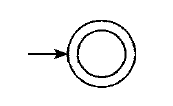
\includegraphics[width=0.2\linewidth]{images/regexp_dim_2}
	\end{center}
	%
	\item $R = \varnothing$. Allora $L(R) = \varnothing$, e il seguente NFA riconosce $L(R)$
	\begin{center}
		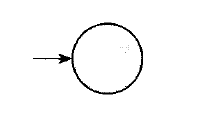
\includegraphics[width=0.2\linewidth]{images/regexp_dim_3}
	\end{center}
	%
	\item $R = R_1 \cup R_2$
	\item $R = R_1 \circ R_2$
	\item $R = R_1^*$
\end{enumerate}
Per gli ultimi tre casi utilizziamo le costruzioni date delle dimostrazioni precedenti, ovvero che i linguaggi regolari sono chiusi rispetto alle operazioni regolari.
\begin{lemma*}
	Se un linguaggio è regolare, allora esiste un'espressione regolare che lo riconosce.
\end{lemma*}
\noindent
Per dimostrare questo lemma abbiamo bisogno di introdurre un nuovo tipo di automa, i GNFA, ovvero un automa a stati finiti non deterministico generalizzato, sui quali archi non vi sono più simboli, ma espressioni regolari.
\pagebreak
\subsection{GNFA}
\example 
\begin{center}
	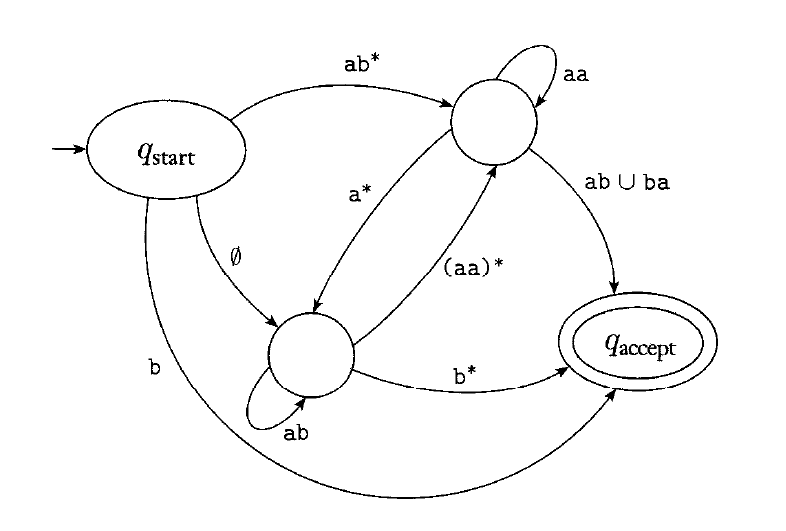
\includegraphics[width=0.7\linewidth]{images/gnfa}
\end{center}
Ci focalizziamo su un GNFA con un formato particolare, ovvero
\begin{enumerate}
	\item Lo stato iniziale ha archi uscenti verso tutti gli altri stati e nessun arco entrante
	\item Lo stato finale ha archi entranti da tutti gli altri stati e nessun arco uscente
	\item Per tutti gli altri stati esiste un arco verso ciascun altro stato, incluso se stesso, ma esclusi quelli finale ed iniziale
\end{enumerate}
Per convertire un DFA in un GNFA ben formato è necessario seguire una serie di passaggi:
\begin{enumerate}
	\item Aggiungi un nuovo stato iniziale con $\varepsilon-$transizioni verso lo stato iniziale originario (il nuovo stato iniziale non ha transizioni in entrata)
	\item Aggiungi uno stato finale, metti $\varepsilon-$transizioni  da ciascuno dei vecchi stati finali verso esso e rendi tali stati non finali
	\item Se una freccia ha più etichette, rimpiazzale con l'unione delle etichette stesse ($a,b \Rightarrow a \cup b$). Se una freccia è mancante, aggiungila ed etichettala con $\varnothing$.
\end{enumerate}
Passaggi tipici di una conversione da GNFA a regular expression:
\begin{center}
	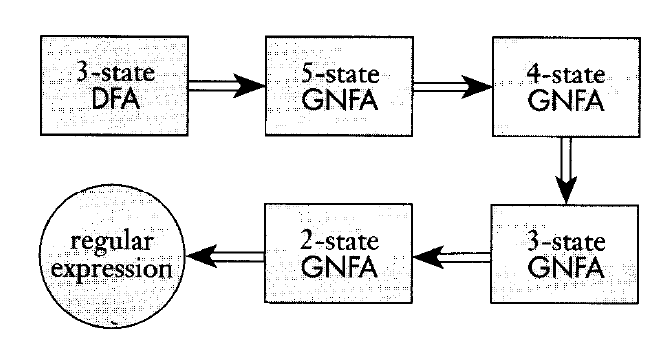
\includegraphics[width=0.5\linewidth]{images/dfa_to_gnfa}
\end{center}
\pagebreak
\example di conversione da DFA a GNFA:
\begin{center}
	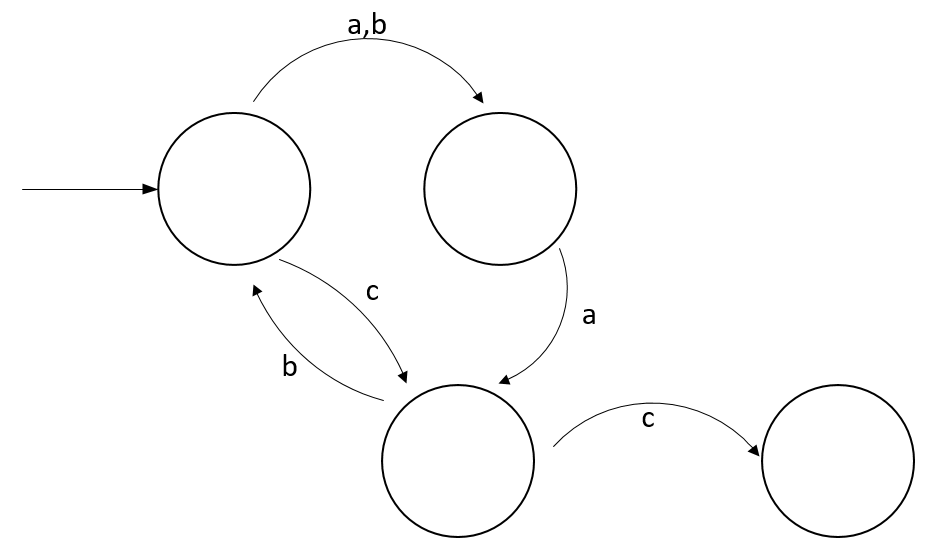
\includegraphics[width=0.5\linewidth]{images/automa9}
\end{center}
\begin{center}
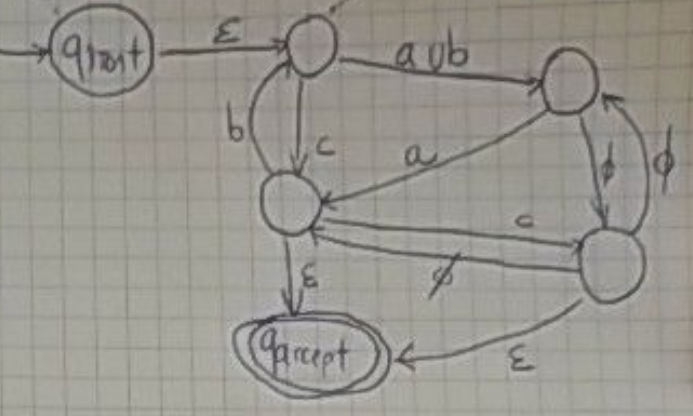
\includegraphics[width=0.5\linewidth]{images/automa10}
\end{center}
\example di normalizzazione di un GNFA, che permette di ridurne gli stati al fine di ottenere un'espressione regolare:
\begin{center}
	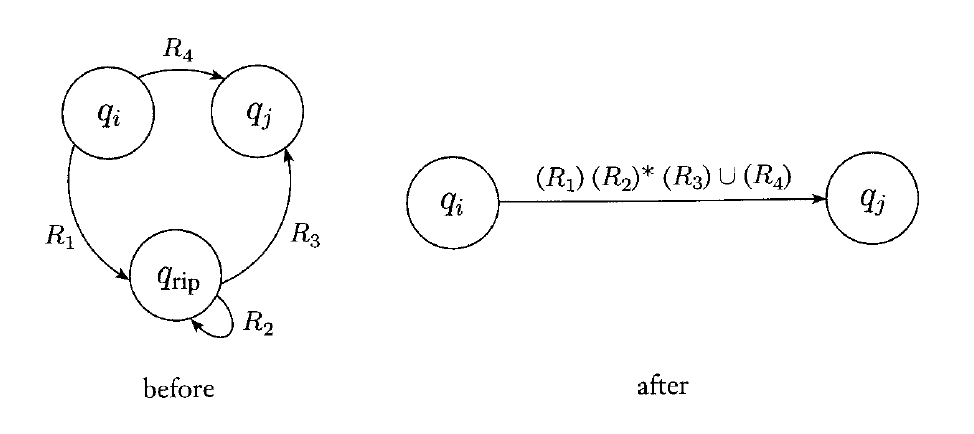
\includegraphics[width=0.5\linewidth]{images/automa12}
\end{center}
\example di normalizzazione di un GNFA:
\begin{center}
	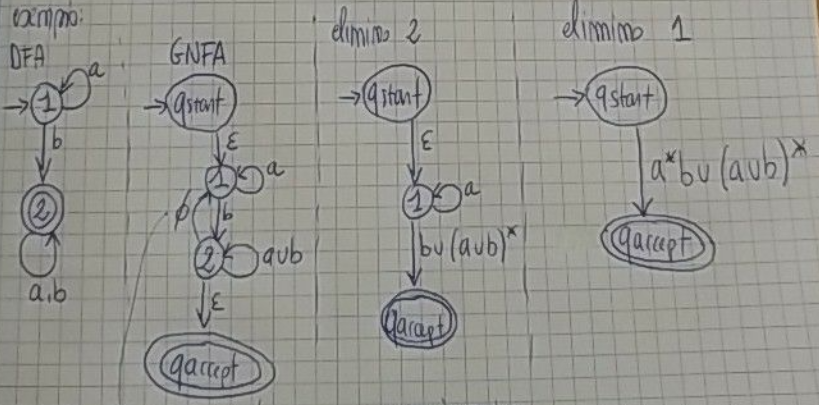
\includegraphics[width=0.7\linewidth]{images/automa11}
\end{center}
\pagebreak
\section{Linguaggi non regolari}
I linguaggi non regolari sono tutti quei linguaggi che non possono essere riconosciuti da nessun automa a stati finiti (DFA).
\begin{gather*}
	A = \{ 0^n1^n \taleche n \geq 0 \} \to \text{non regolare} \\
	A = \{ w \taleche w \text{ ha lo stesso numero di 0 e 1} \} \to \text{non regolare} \\
	A = \{ w \taleche w \text{ ha lo stesso numero di occorrenze delle sottostringhe 01 e 10} \} \to \text{regolare}
\end{gather*}
Andiamo ora a definire uno dei modi che permettono di determinare la regolarità di un linguaggio.
\subsection{Pumping}
\begin{lemma*}
	Se $A$ è un linguaggio regolare, esiste un numero $p$ (pumping length) tale che ogni stringa di $A$ di lunghezza almeno $p$, può essere divisa in tre pezzi $xyz$ tali che
	\begin{enumerate}
		\item $\forall i \geq 0: xy^iz \in A$
		\item $|y| > 0$
		\item $|xy| \leq p$
	\end{enumerate}
\end{lemma*}
\noindent
\textit{Intuizione:} Se $A$ è un linguaggio regolare allora esiste un DFA $M$ che lo riconosce. Imposto $p$ al numero di stati di $M$. Prendiamo una stringa $s$ tale che $|s|>p$. Poiché $|s|>p$ devo attraversare almeno $p+1$ stati per riconoscerla, da qui ricaviamo che uno stato dell'automa deve necessariamente essere attraversato almeno due volte.
\begin{center}
	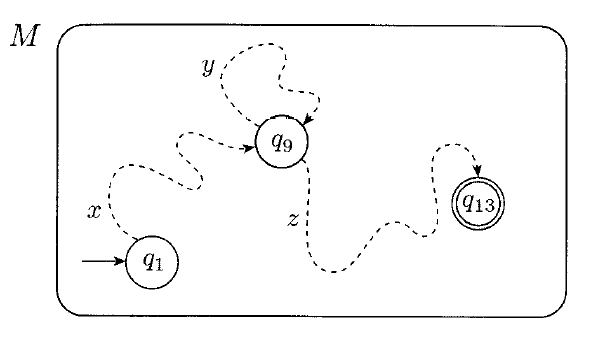
\includegraphics[width=0.3\linewidth]{images/regular_languages_puming}
\end{center}
\begin{proof}
	Sia $A$ un linguaggio regolare, allora esiste un DFA $M$ che lo riconosce. Sia $M = (Q,\;\Sigma,\;\delta,\;q_0,\;F)$ e sia $p$ il numero di stati in $Q$. Sia $s = s_1,\dots,s_n$ tale che $n \geq p$ e sia $r_1,\dots,r_{n+1}$ la sequenza di stati attraversati per riconoscere $s$, allora $r_{i+1} = \delta(r_i,s_i)$. \\
	Tra i primi $p+1$ stati in $r_1,\dots,r_n$ deve esserci una ripetizione, chiamata prima occorrenza $r_j$ e una seconda occorrenza chiamata $r_l$ con $l \leq p+1$. Spezziamo $s$ in tre sotto-stringhe $xyz$ dove:
	\begin{itemize}[label={}]
		\item $x = s_1,\dots,s_{j-1}$
		\item $y = s_j,\dots,s_{l-1}$
		\item $z = s_l,\dots,s_{n}$
	\end{itemize}
	Verifichiamo ora le tre condizioni:
	\begin{enumerate}
		\item $\forall i \geq 0: xy^iz \in A$
		\item $|y| > 0$ \text{ vero perché considero occorrenze diverse dello stato}
		\item Sappiamo che $j \neq l$ e che $l \leq p$, da cui $|xy| \leq p$
	\end{enumerate}
\end{proof}
Per dimostrare che un linguaggio $A$ è non regolare, posso dunque utilizzare il \textit{puming lemma}:
\begin{enumerate}
	\item Assumo per assurdo che $A$ sia regolare
	\item Poiché $A$ è regolare, deve valere il \textit{puming lemma}
	\item Trovo una stringa $s$, con $|s| \geq p$ tale che per ogni particolare $xyz$, con $|xyz|>p$ ho che esiste $i$ tale che $xy^iz \notin A$
	\item Concludo che $A$ non poteva essere regolare
\end{enumerate}
\pagebreak
\example di applicazione del \textit{puming lemma} per verificare la non regolarità di un linguaggio.
\[
	A = \{ 0^n1^n \taleche n \geq 0 \}
\]
Assumo per assurdo che $A$ sia regolare, allora esiste $p$ tale che ogni stringa $s \in A$ può essere scritta come $xyz$ in modo che: $1)\; \forall i \geq 0: xy^iz \in A, \quad 2)\; |y| > 0\quad \text{e}\quad 3)\; |xy| \leq p$. \\\\
Prendo $s = 0^p1^p$ e mostro che $xy^iz \notin A$ per qualche $i$. Procedo per casi:
\begin{enumerate}
	\item $y$ contiene solo $0$. In questo caso $xy^2z \notin A$ perché $xy^2z$ contiene più $0$ che $1$.
	\item $y$ contiene solo $1$. In questo caso $xy^2z \notin A$ perché $xy^2z$ contiene più $1$ che $0$.
	\item $y$ sia $0$ che $1$. 
	\begin{gather*}
		s = 00\underbracket{01}_{y}11 \\
		s = 00\underbracket{0101}_{y^2}11
	\end{gather*}
	In questo caso $xy^2z \notin A$ perché $xy^2z$ conterrà degli $1$ prima di uno $0$.
\end{enumerate}
\example di applicazione del \textit{puming lemma} per verificare la non regolarità di un linguaggio.
\[
	C = \{ w \taleche w \text{ ha lo stesso numero di 0 e 1} \}
\]
Sia $s = 0^p1^p$. Poiché la parte della stringa che vado a pompare deve occorrere nei primi $p$ caratteri di $s$, $y$ deve contenere solo $0$. Perciò $xy^2z$ contiene più $0$ che $1$, da cui $xy^2z \notin C$.\\\\
\example di applicazione del \textit{puming lemma} per verificare la non regolarità di un linguaggio.
\[
	F = \{ ww \taleche w \in \{0,1\}^* \}
\]
Sia $s = 0^p10^p1$. Poiché $|xy| \leq p$, $y$ deve contenere solo $0$, perciò $xy^2z$ contiene più $0$ che $1$, che è lecito, ma rompe la simmetria, da cui $xy^2z \notin F$.\\\\
\example di applicazione del \textit{puming lemma} per verificare la non regolarità di un linguaggio.
\[
	D = \{ 1^{n^2} \taleche n \geq 0 \} \to \text{tutte le stringhe di 1 la cui lunghezza sia un quadrato perfetto}
\]
Sia $s = 1^{p^2} = xyz$, allora $|s| = p^2$. Per il terzo punto del \textit{pumping lemma} ($|xy|\leq p$) impostiamo:
\[
	|xy^2z| = |xyz| + |y|
\]
dove $|xyz| = p^2$, $|y| > 0$ e $|y| < p$.
Quindi
\[
	|xy^2z| \leq p^2 + p < p^2 +2p + 1 = (p+1)^2
\]
perciò , poiché $|y|>0$
\[
	p^2 < |xy^2z| < (p+1)^2
\]
ma allora $|xy^2z|$ non è un quadrato perfetto, e $xy^2z \notin D$.
\pagebreak
\section{Esercizi}
\begin{exercize*}
	Dimostrare che la classe dei linguaggi regolari è chiusa rispetto alla concatenazione. 
	\begin{proof}
		Siano $A$ e $B$ due linguaggi regolari. Poiché sono regolari esisteno due DFA $M$ ed $N$ tali che $L(M) = A$ e $L(N)=B$. Sia $M = (Q_1,\Sigma,\delta_1,q_1,F_1)$ e sia $N = (Q_2,\Sigma,\delta_2,q_2,F_2)$, definisco un DFA $O = (Q,\Sigma,\delta,q_0,F)$ dove:
		\begin{enumerate}
			\item $Q = Q_1 \times Q_2$
			\item $\delta((q_1,q_2),a) = (\delta_1(q_1,a),\delta_2(q_2,a))$
			\item $q=(q_1,q_2)$
			\item $F=\{(q_1,q_2) \taleche q_1 \in F_1 \land q_2 \in F_2\} = F_1 \times F_2$
		\end{enumerate}
	\end{proof}
\end{exercize*}
\begin{exercize*}
	Dimostrare che $C=\{ w \taleche w \text{ ha lo stesso numero di 0 e 1}\}$ non è regolare, senza utilizzare il \textit{pumping lemma}.
	\begin{proof}
		Per assurdo assumo che $C$ sia regolare. Poiché i linguaggi regolari sono chiusi rispetto all'intersezione, la seguente intersezione
		\[
			C \cap 0^*1^*
		\]
		dovrebbe essere regolare. Ma $C \cap 0^*1^* = \{ 01^n \taleche n \geq 0 \}$ e questo non è regolare, da cui $C$ è non regolare. 
	\end{proof}
\end{exercize*}
\begin{exercize*}
	Dimostrare che il linguaggio $D=\{ w \taleche w \text{ lo stesso numero di sottostringhe 01 e 10 }\}$ è regolare.
	\begin{proof}
		Costruisco un DFA che non ho voglia di inserire...
	\end{proof}
\end{exercize*}
\begin{exercize*}
	Dimostrare che i linguaggi regolari sono chiusi rispetto all'operazione di complemento $\bar{A} = \{ w \taleche w \notin A \}$.
	\begin{proof}
			Sia $A$ un linguaggio regolare. Allora esiste un DFA $M = (Q,\Sigma,\delta,q_0,F)$ tale che $L(M) = A$. Costruisco un altro DFA $N = (Q,\Sigma,\delta,q_0,\nicefrac{Q}{F})$, e osservo che $L(N) = \bar{A}$.
	\end{proof}
\end{exercize*}
\begin{exercize*}
	Dimostrare che il linguaggio $B=\{ w \taleche w \text{ non contiene la stringa ab }\}$ è regolare.
	\begin{proof}
		Costruisco un DFA $N$ tale che $L(N) = \{ w \taleche w \text{ contiene la stringa ab }\}$. Poiché $B = \bar{L(N)}$ concludo la chiusura rispetto al complemento che $B$ è regolare.
	\end{proof}
\end{exercize*}
\begin{exercize*}
	Dimostrare che il linguaggio $E=\{ 0^i1^j \taleche i > j \}$ è non regolare.
	\begin{proof}
		Assumo per assurdo che $E$ sia regolare, allora esiste $p$ tale che ogni stringa $s \in E$ è tale che $|s| > p$ può essere scritta come $xyz$ dove:
		\begin{enumerate}
			\item $\forall i xy^iz \in E$
			\item $|y| > 0$
			\item $|xy| \leq p$
		\end{enumerate} 
	Prendo $s = o^{p+1}1^p$. Poiché $|xy| \leq p$, so che $y$ comprende solo $0$. La stringa $xy^0z \notin E$, perché essa comprende meno di $p+1$ zeri:
	\[
	\overbracket{\underbracket{0...0}_{x}}^{p+1}\underbracket{0}_{y}\overbracket{\underbracket{1...1}_{z}}^{p}
	\]
	\end{proof}
\end{exercize*}
\section{Context-free languages}
In questo capitolo introdurremo le grammatiche \textit{context-free}, un metodo più potente per descrivere linguaggi.
\subsection{Context-free grammars}
Il seguente è un esempio di una grammatica \textit{context-free}, che chiameremo $G_1$:
\begin{gather*}
	A \to 0A1 \\
	A \to B \\
	B \to \#
\end{gather*}
Una grammatica consiste in una collezione di \textit{regole di sostituzione}, anche chiamate \textbf{produzioni}. Ogni regola appare come una linea e comprende un \textit{simbolo} e una stringa, separati da una freccia. Il simbolo è chiamato \textbf{variabile}, mentre le stringhe consistono in altre variabili e simboli, chiamati \textbf{terminali}. I simboli delle variabili spesso sono rappresentate in lettere maiuscole, mentre i terminali sono analoghi all'alfabeto di input e sono spesso rappresentati da lettere minuscole, numeri o caratteri speciali. Una tra le variabili della grammatica è la \textbf{variabile di start}, e solitamente si trova a sinistra della regola più in alto. \\

\noindent
La grammatica $G_1$ contiene dunque tre produzioni (le tre righe), le sue variabili sono $A$ e $B$, dove $A$ è la variabile di start. I sui terminali sono $0$, $1$ e $\#$. \\

\noindent
Si utilizza una grammatica per descrivere un linguaggio generando ogni stringa di quel linguaggio nel seguente modo:
\begin{enumerate}[itemsep=0pt]
	\item Si scrive la variabile di start
	\item Si seleziona una della variabili disponibili e la si riscrive come parte destra di una produzione per quella variabile
	\item Si torna al punto 2 fino a che ci sono ancora variabili disponibili
\end{enumerate}
Per esempio la grammatica $G_1$ genera la stringa $000\#111$. La sequenza di sostituzioni per ottenere la stringa viene detta \textbf{derivazione}. La derivazione della stringa $000\#111$ nella grammatica $G_1$ é
\[
	A \Rightarrow 0A1  \Rightarrow 00A11 \Rightarrow 000A111 \Rightarrow 000B111 \Rightarrow 000\#111
\]
Tutte le stringhe generate in questo modo costituiscono il \textit{linguaggio della grammatica}. Indichiamo con $L(G_1)$ il linguaggio della grammatica $G_1$, che è formalmente definito come $\{ 0^n\#1^n \taleche n \geq 0 \}$. Ogni linguaggio che può essere generato da una grammatica \textit{context-free} è chiamato \textit{context-free language \nolinebreak (CFL)}.\\

\noindent
Un altro modo per indicare visivamente una grammatica \textit{context-free} sono i \textit{parse tree}
\begin{center}
	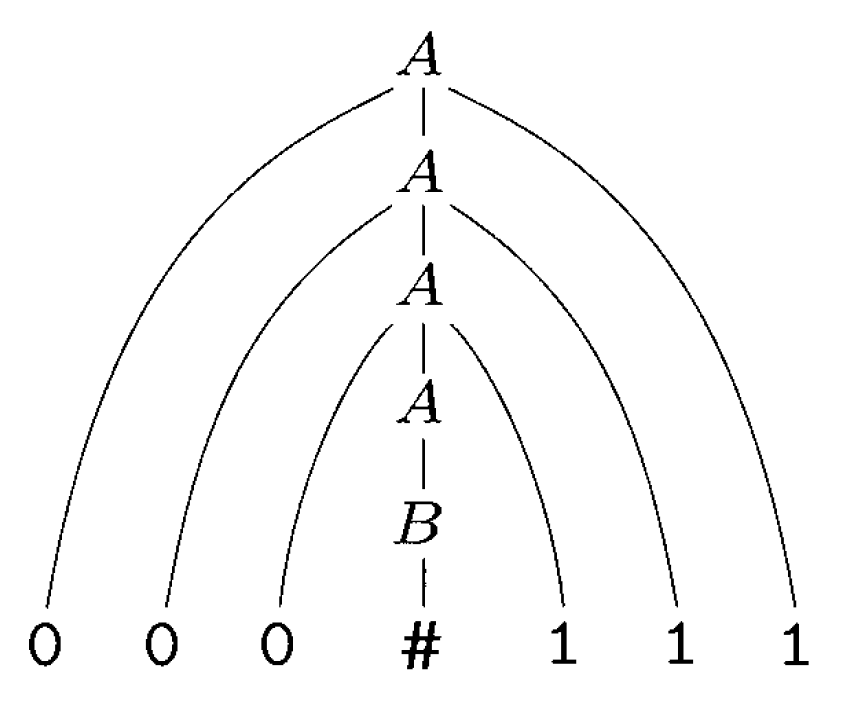
\includegraphics[width=0.3\linewidth]{images/parse_tree}
\end{center}
dove la radice rappresenta la start variable, le foglie i terminali e i nodi intermedi sono dettati dalle produzioni.
\pagebreak
\subsubsection{Definizione}
Una grammatica context-free è una $4$-tupla $(V,\;\Sigma,\;R,\;S)$ dove
\begin{enumerate}
	\item $V$ è un insieme finito di variabili
	\item $\Sigma$ è un insieme finito, disgiunto da $V$, di terminali
	\item $R$ è un insieme finito di regole (produzioni), dove ogni produzione ha la forma $A \to w$ dove $A \in V$ e $w \in (\Sigma \cup V)^*$, ovvero che $w$ può essere una stringa di terminali e/o variabili
	\item $S \in V$ è la start variable
\end{enumerate}
Siano $u,v,w \in (\Sigma \times V)^*$ e sia $A \to w$ una produzione. Diciamo che $uAv$ produce $uwv$ $(uAv \Rightarrow uwv)$. Diciamo che $u$ deriva da $v$ $(u \derive v)$ sse $u=v$ oppure $\exists w_1,\dots,w_n \taleche u \Rightarrow w_1 \Rightarrow \dots \Rightarrow w_n \Rightarrow v$.  \\

\noindent
Data una grammatica $G = (V,\;\Sigma,\;R,\;S)$, definiamo il linguaggio generato da $G$ come l'insieme delle stringhe di terminali derivabili dalla start variable:
\[
	L(G) = \{ w \in \Sigma^* \taleche S \derive w \}
\]

\example Dato $G = (\{S\},\{a,b\},R,S)$, dove $R$ è definito da $S \to aSb \taleche SS \taleche \varepsilon$, determinare alcune stringhe che può comporre.
\begin{itemize}
	\item $abab: \qquad S \To SS \To aSbS \To abS \To abaSb \To abab$
	\item $aabb: \qquad S \To aSb \To aaSbb \To aabb$
\end{itemize}
Supponendo quindi che $a$ rappresenti la parentesi sinistra "(" e $b$ quella destra ")", il linguaggio di $G$ è quello di tutte le stringhe le cui parentesi siano annidate correttamente. \\

\example Generare il \textit{parse tree} che generi $a+a\times a$ dati
\begin{itemize}
	\item $E \To E + T \taleche T$
	\item $T \To T \times F \taleche F$
\end{itemize}
\begin{center}
	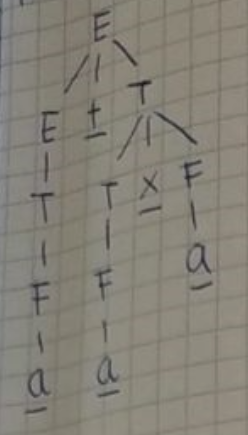
\includegraphics[width=0.3\linewidth]{images/parse_tree_1}
\end{center}
\pagebreak
\subsubsection{Ambiguità}
Una grammatica è \textit{ambigua} se e solo se esiste $w \in L(G)$ con almeno due \textit{leftmost} diversi. Per \textit{leftmost} si s'intende che nel processo di derivazione ( e di conseguenza nel \textit{parse tree}) scrivo il terminale a sinistra.\\

\example Dato $E \to E+E \taleche E \times E \taleche a \taleche (E)$, verificare che sia ambiguo.\\

\noindent 
A questo punto sviluppo due \textit{parse tree}, e dal momento che ottengo la stessa stringa "$a+a\times a$" in due modi differenti, concludo che la grammatica è ambigua.
\begin{center}
	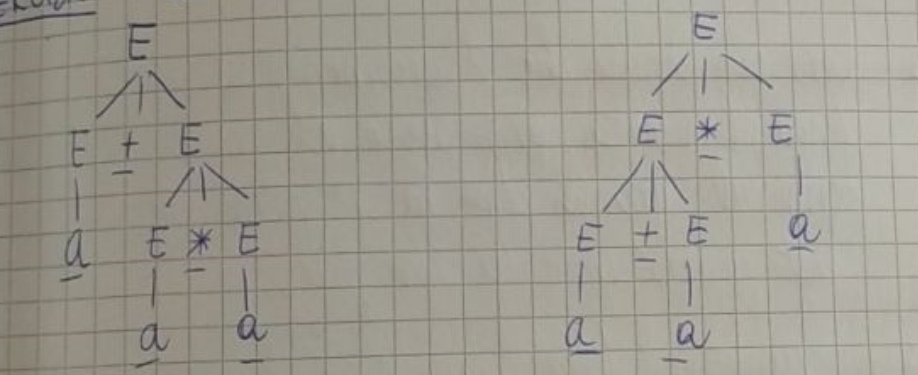
\includegraphics[width=0.5\linewidth]{images/parse_tree_2}
\end{center}
\subsection{Forma normale di Chomsky}
Un \textit{context-free language} è in forma normale di Chomsky se ogni sua produzione ha la forma $A \to BC$ oppure $A \to a$ con l'eccezione che $B,C$ non possono essere la variabile di start. Inoltre ammettiamo $S \to \varepsilon$ dove $S$ è la start variable.

\begin{theorem*}
	Ogni linguaggio context-free è generabile da una grammatica context-free in forma normale di Chomsky. [vedi pag 99, theorem 2.6]
	\begin{proof}
		Definiamo un algoritmo per convertire una CFG qualsiasi in forma normale:
		\begin{enumerate}
			\item Sia $S$ lo start symbol, invento un nuovo start symbol $S' \to S$
			\item Sia $A \to \varepsilon$ una $\varepsilon$-produzione con $A \neq S$. Allora cancello $A \to \varepsilon$ e in tutti i punti in cui $A$ occorre, aggiungo una nuova produzione dove $A$ è cancellata per ogni possibile occorrenza di $A$, ovvero
				\begin{gather*}
			\begin{flalign*}
			R \to uAwAv \rightsquigarrow & R \to uAwAv \text{ non cancello occorrenze di $A$} & \\
			& R \to uwAv \text{ cancello 1 occorrenza di $A$} \\
			& R \to uAwv \text{ cancello 2 occorrenze di $A$} \\
			& R \to uwv \text{ cancello 3 occorrenze di $A$} 
			\end{flalign*}
			\end{gather*}
			Se avessi
			\begin{gather*}
			\begin{flalign*}
			R \to A \rightsquigarrow & R \to A & \\
			& R \to \varepsilon 
			\end{flalign*}
			\end{gather*}
			\item Elimina le produzioni unitarie della forma $A\to B$ se esiste $A\to B$ e $B \to w_1 \taleche \dots \taleche w_n$, cancella $A\to B$ e sostituiscilo con $A \to w_1 \taleche \dots \taleche w_n$.
			\item A questo punto tutte le produzioni della grammatica hanno almeno due simboli a destra.
			\item Nelle regole precedenti rimpiazzo ogni terminale $u_i$ con $1 \leq i \leq k$ con un non terminale $U_i$ e aggiungi $U_i \to u_i$
		\end{enumerate}
	\end{proof}
\end{theorem*}
\pagebreak
\example Normalizzazione il CFG $G$ nella forma normale di Chomsky. 
\begin{enumerate}
	\item Il CFG è mostrato sulla sinistra. Il risultato dell'applicazione del primo step per creare un nuovo start symbol appare sulla destra.
		\begin{gather*}
			\begin{align*}
				\begin{split}
					& A \to ASA \taleche aB \\
					& A \to B \taleche S \\
					& B \to b \taleche \varepsilon
				\end{split}
				&
				\begin{split}
					& S_0 \to S \\
					& A \to ASA \taleche aB \\
					& A \to B \taleche S \\
					& B \to b \taleche \varepsilon
				\end{split}
			\end{align*}
		\end{gather*}
	\item Rimuovendo le $\varepsilon$-produzioni $B \to \varepsilon$ sulla sinistra, e $A \to \varepsilon$ sulla destra:
		\begin{gather*}
		\begin{align*}
		\begin{split}
		& S_0 \to S \\
		& S \to ASA \taleche aB \taleche a \\
		& A \to B \taleche S \taleche \varepsilon \\
		& B \to b \taleche \varepsilon
		\end{split}
		&
		\begin{split}
		& S_0 \to S \\
		& S \to ASA \taleche aB \taleche a \taleche SA \taleche AS \taleche S\\
		& A \to B \taleche S \taleche \varepsilon \\
		& B \to b 
		\end{split}
		\end{align*}
		\end{gather*}
	\item Rimuovendo le produzioni unitarie $S \to S$, sulla sinistra e $S_0 \to S$ sulla destra:
			\begin{gather*}
	\begin{align*}
	\begin{split}
	& S_0 \to S \\
	& S \to ASA \taleche aB \taleche a \taleche SA \taleche AS \taleche S \\
	& A \to B \taleche S \\
	& B \to b
	\end{split}
	&
	\begin{split}
	& S_0 \to S \taleche ASA \taleche aB \taleche a \taleche SA \taleche AS \\
	& S \to ASA \taleche aB \taleche a \taleche SA \taleche AS \\
	& A \to B \taleche S\\
	& B \to b 
	\end{split}
	\end{align*}
	\end{gather*}
	\item Rimuovendo le produzioni unitarie $A\to B$ e $A\to S$:
	\begin{gather*}
	\begin{align*}
	\begin{split}
	& S_0 \to ASA \taleche aB \taleche a \taleche SA \taleche AS \\
	& S \to ASA \taleche aB \taleche a \taleche SA \taleche AS \\
	& A \to B \taleche S \taleche b \\
	& B \to b
	\end{split}
	&
	\begin{split}
	& S_0 \to ASA \taleche aB \taleche a \taleche SA \taleche AS \\
	& S \to ASA \taleche aB \taleche a \taleche SA \taleche AS \\
	& A \to S \taleche b \taleche ASA \taleche aB \taleche a \taleche SA \taleche AS \\
	& B \to b
	\end{split}
	\end{align*}
	\end{gather*}
	\item Convertiamo le produzioni rimanenti nella forma corretta aggiungendo le variabili e le produzioni necessarie. Il risultato finale è
		\begin{gather*}
	S_0 \to AA_1 \taleche UB \taleche a \taleche SA \taleche AS \\
	S \to AA_1 \taleche UB \taleche a \taleche SA \taleche AS \\
	A \to B \taleche AA_1 \taleche UB \taleche a \taleche SA \taleche AS \\
	A_1 \to SA \\
	U \to a \\
	B \to b
	\end{gather*}
\end{enumerate}

\pagebreak
\subsection{Push-down automata}
In questa sezione introdurremo i \textit{pushdown automata}. Questi automi sono simili agli automi finiti non deterministici, ma hanno un componente in più chiamato stack. Lo stack fornisce memoria addizionale a quella finita disponibile ni NFA. Lo stack permette dunque a questi speciali automi di riconoscere alcuni linugaggi non regolari. Gli autocmi \textit{pushdown} sono equivalenti in espressività alle grammatiche \textit{context-free}.
\begin{center}
	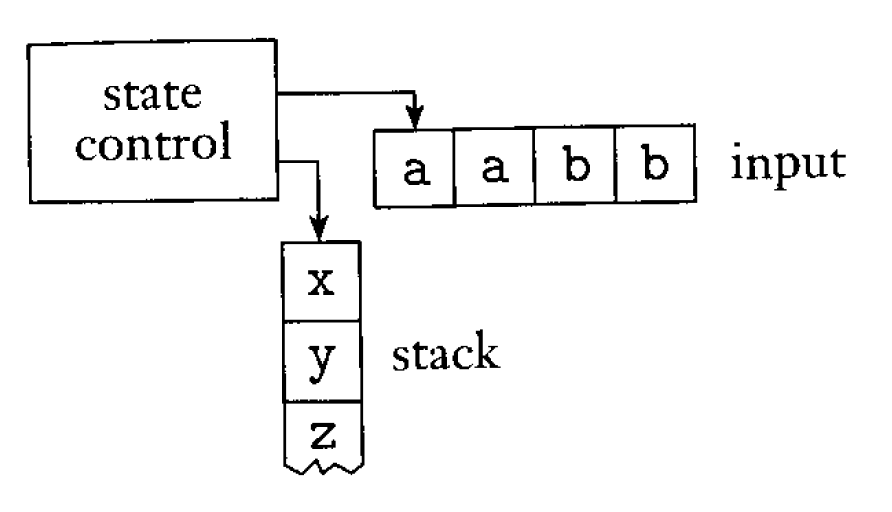
\includegraphics[width=0.4\linewidth]{images/pushdown_automata}
\end{center}
Notiamo che l'alfabeto dello stack e di input possono essere differenti.
\subsubsection{Definizione}
Un automa \textit{pushdown} è una $6$-tupla $(Q,\;\Sigma,\;\varGamma,\;\delta,\;q_0,\;F)$ dove
\begin{enumerate}
	\item $Q$ è un insieme finito di stati
	\item $\Sigma$ è un insieme finito di simboli di input
	\item $\varGamma$ è un insieme finito di simboli per lo stack
	\item $\delta: Q \times (\Sigma \cup \{\varepsilon\})\times(\varGamma \cup \{ \varepsilon\}) \to \powerset{Q \times (\varGamma \cup \{\varepsilon\})}$
	\item $q_0 \in Q$ è lo stato iniziale
	\item $F \subseteq Q$ è l'insieme degli stati finali
\end{enumerate}
Un PDA $M = (Q,\;\Sigma,\;\varGamma,\;\delta,\;q_0,\;F)$ accetta l'input $w$ se $w$ si può scrivere come $w_1w_2...w_n$ dove $\forall i \; w_i \in \Sigma \cup \{\varepsilon\}$ (ovvero come negli NFA posso avere $\varepsilon$-transizioni spontanee) ed esiste una sequenza di stati $r_0,r_1,\dots,r_n \in Q$ e stack $s_0,s_1,\dots,s_n \in \varGamma^*$ tali che:
\begin{enumerate}
	\item $r_0 = q_0$ e $s_0 = \varepsilon$, ovvero che $M$ inizia nello stato iniziale e con lo stack vuoto
	\item $r_n \in F$, ovvero che $M$ finisce di computare in uno stato accettante dopo aver concluso di leggere l'input
	\item $\forall i \in [0,n-1]:\;(r_{i+1},b) \in \delta(r_1,w_{i+1},a)$ dove $s_i = at$ e $s_{i+1} = bt$ per qulche $a,b \in \varGamma \cup \{\Sigma\}$ e $t \in \varGamma^*$. Ovvero che per tutti gli stati, lo stato successivo ($r_{i+1}$) è calcolato dallo stato precedente e dal successivo simbolo di input ($\delta(r_i,w_{i+1})$). Però in ogni momento posso leggere un simbolo dallo stack e aggiornare lo stato dello stack. Quindi valuto sia chi transita dallo stato sia il carattere $a$ in cima allo stack dello stato corrente nel tempo $i$ (enllo stato $r_i$). Nello stato successivo voglio aggiornare $a$ con $b$ (pop di $a$ e push di $b$). Però non vengono sempre fatte push e pop perché possono esserci anche le $\varepsilon$-transizioni e al posto di $a$ e $b$ possono esserci tre casi:
	\begin{enumerate}
		\item $a=\varepsilon,b \neq \varepsilon$: push
		\item $a\neq\varepsilon,b = \varepsilon$: pop
		\item $a=\varepsilon,b =\varepsilon$: non modifico lo stack, ma faccio un $\varepsilon$-transizione
	\end{enumerate}
\end{enumerate}
\pagebreak
\example Trovare un PDA che riconosca il linguaggio $\{ 0^n1^n \taleche n \geq 0 \}$. \\

\noindent
L'idea è che se leggo $0$ riempio lo stack, mentre leggendo $1$ lo svuoto. Mantengo un simbolo di flag ($\$$) che mi indica quando lo stack è vuoto, e quando arrivo alla fine dell'input se lo stack è vuoto significa che l'input viene riconosciuto.
\begin{center}
	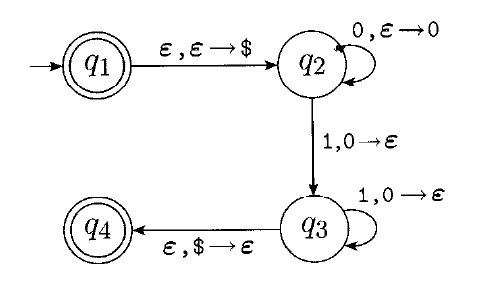
\includegraphics[width=0.4\linewidth]{images/pda}
\end{center}
Quando scriviamo $a,b \to c$ significa che quando l'automa sta leggendo un $a$ dall'input, può rimpiazzare il simbolo $b$ nella testa dello stack con il simbolo $c$. Sia $a$ che $b$ e $c$ possono essere $\varepsilon$. Se $a = \varepsilon$, l'automa esegue la transizione senza leggere nessun simbolo dall'input. Se $b=\varepsilon$ l'automa può eseguire la transizione senza leggere dall'input e prendere il primo simbolo dallo stack. Se $c=\varepsilon$ l'automa non scrive nessun simbolo nello stack eseguendo questa transizione. \\

\example Determinare il PDA che riconosce il linguaggio
\[
	\{ ww^R \taleche w \in \{0,1\}^* \}\qquad \text{dove } w^R \text{ equivale ad $w$ rovesciato (reverse)}
\]
Il DFA deve riconoscere quindi, ad esempio, la stringa $\underbracket{100}_{w}\overbracket{001}^{w^R}$
\begin{center}
	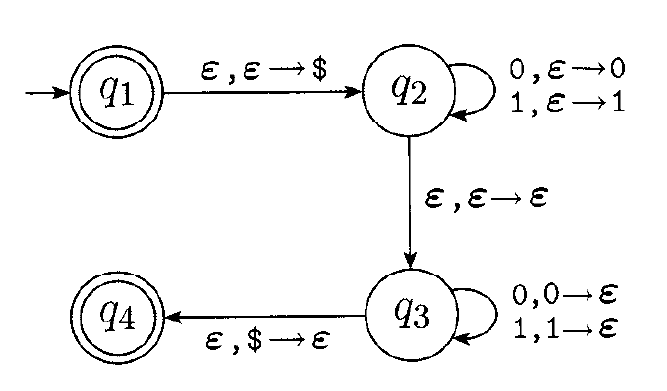
\includegraphics[width=0.4\linewidth]{images/pda-1}
\end{center}

\begin{theorem*}
	Un linguaggio è \textit{context-free} se e solo se è riconosciuto da un PDA.
	\begin{proof}
		Se un linguaggio è \textit{context-free} allora è riconosciuto da un PDA. Intuitivamente, se esiste un linguaggio è \textit{context-free}, esiste una grammatica $G$ che lo genera. Diamo una definizione informale del PDA:
		\begin{enumerate}
			\item Metti sullo stack "\$" seguito da $S$, dove $S$ è lo \textit{start symbol} della grammatica
			\item Ripeti i seguenti passi
				\begin{enumerate}
					\item Se in cima allo stack ho $A$, scegli una produzione $A \to w$ e sostituisci $A$ con $w$
					\item Se in cima allo stack ho $a$, confrontalo con il prossimo carattere in input e fai la pop se sono uguali, fallisci termina questo ramo del non determinismo
					\item Se in cima allo stack ho "\$" ed ho finito l'input, accetta
				\end{enumerate}
		\end{enumerate}
		Per semplificare la definizione che andremo a vedere, occorre introdurre una notazione sharthand, più compatta, che ci permette di fare il push di stringhe intere anziché di singoli caratteri.
		\begin{center}
			\begin{figure}[h]
				\centering
				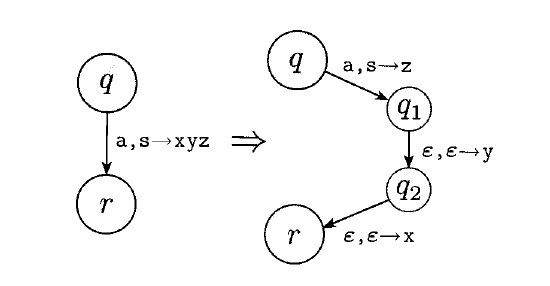
\includegraphics[width=0.5\linewidth]{images/pda-shorthand}
				\caption[Implementazione della shorthand $(r,xyz) \in \delta(q,a,s)$]{Implementazione della shorthand $(r,xyz) \in \delta(q,a,s)$}
				\label{fig:pda-shorthand}
			\end{figure}
	\end{center}
	Sia l'immagine lo schema che ci permette di fare il push di una stringa e sia $E$ l'insieme degli stati ausiliari utilizzati per simulare le transizioni necessarie per pushare una stringa e non un carattere. \\
	
	\noindent
	Sia $Q = \{q_{start},q_{loop},q_{accept}\} \cup E$ e sia definita la funzione di transizione come
	\begin{gather*}
		\delta(q_{start},\varepsilon,\varepsilon) = \{ q_{loop}, S\$ \} \\
		\delta(q_{loop},\varepsilon,A) = \{ q_{loop}, w \taleche A \to w \text{ è una produzione} \} \\
		\delta(q_{loop},a,a) = \{ q_{loop}, \varepsilon \} \\
		\delta(q_{loop},\varepsilon,\$) = \{ q_{accept}, \varepsilon \} 
	\end{gather*}
	\begin{center}
		\begin{figure}[h]
			\centering
			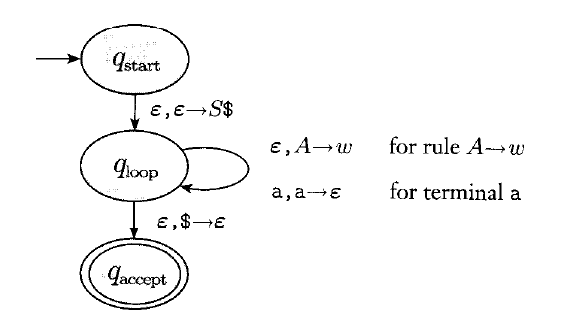
\includegraphics[width=0.5\linewidth]{images/pda-delta}
			\caption[Diagramma di stato di $Q$]{Diagramma di stato di $Q$}
			\label{fig:pda-delta}
		\end{figure}
	\end{center}
	\end{proof}
	\begin{proof}
		Se un li linguaggio è riconoscibile da un PDA, allora è \textit{context-free}. Ci focalizziamo su un PDA con tre caratteristiche:
		\begin{enumerate}
			\item Ha un unico stato finale $q_{accept}$
			\item Svuota lo stack prima di accettare
			\item Ogni transizione è o una push o una pop, ma mai entrambe contemporaneamente
		\end{enumerate} 
		L'idea è che per ogni coppia di stati $p$ e $q$ del PDA, invento una variabile $A_{pq}$ che genera tutte le stringhe che portano il PDA da $p$ a $q$ con lo stack vuoto. Quindi dato un input $x$ il PDA farà come prima mossa una push e come ultima mossa una pop, dal momento che inizio e termino con lo stack vuoto.
		\begin{itemize}
			\item Se il carattere che poppo alla fine è lo stesso che ho pushato all'inizio, lo stack non si è mai svuotato. Simulo con 
			\begin{gather*}
				a = \text{primo carattere letto} \\
				b = \text{ultimo carattere letto} \\
				r = \text{stato dopo di $p$} \\
				s = \text{stato prima di $q$} \\
			\end{gather*}
			allora 
			\[
				A_{pq} \to aA_{rs}b
			\]
			\begin{center}
				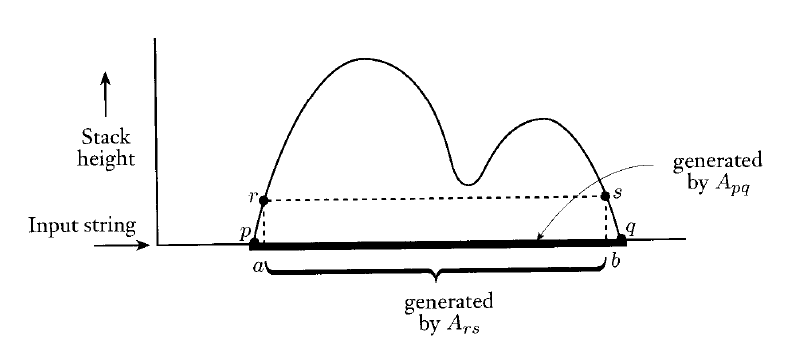
\includegraphics[width=0.7\linewidth]{images/pda-ars}
			\end{center}
			\item Altrimenti esiste uno stato $r$ dove lo stack si è svuotato. Simulo con:
			\[
				A_{pq} \to A_{pr}A_{rq}
			\]
			\begin{center}
				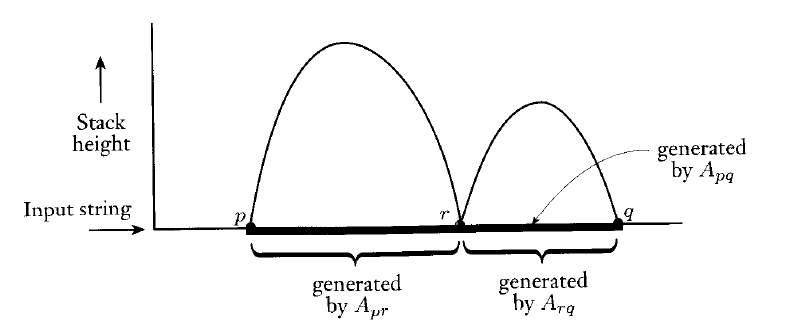
\includegraphics[width=0.7\linewidth]{images/pda-apr}
			\end{center}
		\end{itemize}
	\end{proof}
\end{theorem*}
	\noindent
	Sia $P = (Q,\Sigma,\varGamma,\delta,q_0,\{q_{accept}\})$ un PDA delle forma specificata. Le variabili della grammatica sono 
	\[
		\{ A_{pq} \taleche p,q \in Q\}
	\]
	mentre le produzioni sono
	\begin{enumerate}
		\item Per ogni $p,q,r,s \in Q$ e per ogni $a,b \in \Sigma \cup \{\varepsilon\}$, se $(r,u) \in \delta(p,a,\varepsilon)$ e $(q,\varepsilon) \in \delta(s,b,u)$
		\item Per ogni $p,q,r,s \in Q$, aggiungi $A_{pq} \to A_{pr}A_{rq}$
		\item Per ogni $p \in Q$ aggiungi $A_{pp} \to \varepsilon$
	\end{enumerate}
	%% Puming Lemma per CFL
	\subsection{Pumping lemma per CFL}
	Se $A$ è un linguaggio \textit{context-free} esiste un numero $p$ (\textit{pumping length}) tale che per ogni $i \in A$ tale che $\len{s} \geq p$ abbiamo che $s = uvxyz$, dove:
	\begin{enumerate}
		\item $\forall i \geq 0 : uv^ixy^iz \in A$
		\item $|vy| > 0$
		\item $|vxy| \leq p$		
	\end{enumerate}
	\subsubsection{Proof idea}
	Sia $A$ un linguaggio \textit{context-free} e sia $G$ una \textit{context-free grammar} che lo descrive. Dobbiamo dimostrare che qualunque stringa sufficientemente lunga può essere pompata e rimanere in $A$.\\
	
	\noindent
	Sia $s$ una stringa molto lunga in $A$ (dopo definiremo il quanto lunga). Poiché $s \in A$ è derivabile da $G$, ha un \textit{parse-tree}. Il \textit{parse-tree} deve essere molto alto in quanto $s$ è molto lunga. Il \textit{parse-tree} deve dunque contenere un cammino dalla \textit{start variabile} alla radice dell'albero ad un simbolo terminale in una foglia. In questo lungo cammino qualche variabile $R$ deve ripetersi per il \href{https://it.wikipedia.org/wiki/Principio_dei_cassetti}{principio dei cassetti}. Come mostra le figura seguente questa ripetizione ci permette di rimpiazzare il sottoalbero sotto la seconda occorrenza di $R$ con il sottoalbero sotto la prima occorrenza di $R$ e continuare ad avere un \textit{parse-tree} valido e legale. \\
	
	\noindent
	Pertanto possiamo dividere $s$ in cinque pezzi $vuxyz$ come indica la figura, e possiamo ripetere il secondo e il quarto pezzo ottenendo una stringa ancora nel linguaggio. In altre parole $uv^ixy^iz \in A \; \forall i \geq 0$. 
	\begin{figure}[h]
		\centering
		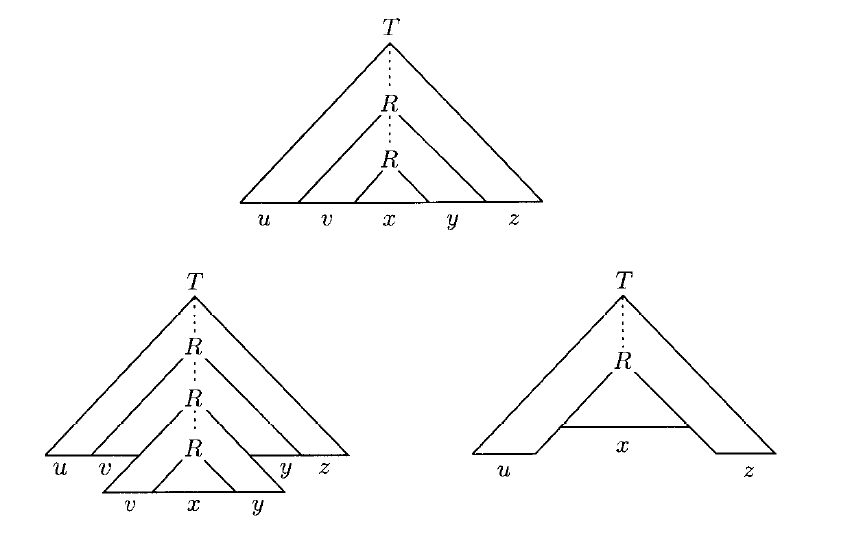
\includegraphics[width=0.7\linewidth]{images/parse_tree_cfl}
		\caption[Rimpiazzamento dei \textit{parse-tree}]{Rimpiazzamento dei \textit{parse-tree}}
		\label{fig:parsetreecfl}
	\end{figure}

	\noindent
	Andiamo ora a definire i dettagli per ottenere le tre condizioni del \textit{pumping lemma} e per calcolare il \textit{pumping length}~$p$.
	\pagebreak
	\subsubsection{Dimostrazione}
	Sia $G$ una CFG per il CFL $A$. Sia $b$ la lunghezza massima dei simboli nella parte destra delle produzioni, per assunzione $b \geq 2$. In ogni \textit{parse-tree} utilizzando questa grammatica sappiamo che un nodo non può avere più di $b$ figli. In altre parole al massimo $b$ foglie sono alla distanza di $1$ passo dalla radice; al massimo $b^2$ foglie sono al massimo a $2$ passi dalla radice; al massimo $b^h$ foglie sono al massimo a $h$ passi dalla radice.Quindi se l'altezza del \textit{parse-tree} è al massimo $h$, la lunghezza della stringa generata è al massimo $b^h$. \\
	
	\noindent
	Sia $\len{V}$ il numero di variabili in $G$. Definiamo $p = b^{\len{V}+2}$. Poiché $b \geq 2$, sappiamo che $p > b^{\len{V}+1}$, quindi un \textit{parse-tree} per una stringa di $A$ di lunghezza almeno $p$ richiede un'altezza di almeno $\len{V} + 2$. Supponiamo che $s$ sia una stringa di $A$ con lunghezza almeno $p$. Ora mostreremo come pompare $s$. \\
	
	\noindent
	Sia $\tau$ un \textit{parse-tree} per $s$. Se $s$ ha più di un \textit{parse-tree} prendiamo in considerazione quello con il minor numero di nodi. Siccome $\len{s} > p$, sappiamo che $\tau$ ha altezza almeno $\len{V}+2$, quindi il cammino più lungo è di lunghezza almeno $\len{V}+2$. Questo cammino deve avere almeno $\len{V}+1$ variabili in quando solo la foglia è terminale. Con $G$ che ha solo $\len{V}$ variabili, qualche variabile $R$ appare più di una volta nel cammino. Per convenienza prendiamo $R$ in modo che sia la variabile che si ripete nelle $\len{V}+1$ variabili più in basso nel cammino. \\
	
	\noindent
	Dividiamo $s$ come mostrato in Figura~\ref{fig:parsetreecfl}. Ogni occorrenza di $R$ ha un sottoalbero sotto di essa, generando così una parte della stringa $s$. L'occorrenza più in alto di $R$ ha un sottoalbero più grande e genera $vxy$, mentre l'occorrenza più in basso genera solo $x$ con un sottoalbero più piccolo. Entrambi questi sotto-alberi sono generati dalla stessa variabile, quindi noi potremmo sostituirli uno con l'altro e ottenere comunque un \textit{parse-tree} valido. Rimpiazzando il sottoalbero più piccolo con quello più grande ripetutamente otteniamo un \textit{parse-tree} che genera le stringhe $uv^ixy^iz \; \forall i > 1$. Rimpiazzando il più grande con il più piccolo otteniamo invece la stringa $uxz$. Questo soddisfa la condizione 1 del pumping lemma. Andiamo ora a vedere come soddisfare le altre due condizioni.\\
	
	\noindent
	Per ottenere la condizione 2 dobbiamo essere sicuri che entrambi $v$ e $y$ siano non $\varepsilon$. Se lo fossero il parse-tree ottenuto sostituendo il sottoalbero più piccolo con quello più grande avrebbe meno nodi di $\tau$ e genererebbe comunque $s$. Ma questo è impossibile in quanto avevamo già scelto il parse-tree in modo che fosse quello con il minor numero di nodi. \\
	
	\noindent
	Per soddisfare il punto 3 dobbiamo essere sicuri che $vxz$ abbia lunghezza al massimo $p$. Nel parse-tree di $s$ l'occorrenza più in alto di $R$ genera $vxz$. Abbiamo scelto $R$ in modo che entrambe le occorrenze fossero nelle $\len{V}+1$ variabili più in basso del cammino, e abbiamo scelto il più lungo cammino nel parse-tree, quindi il sottoalbero dove $R$ genera $vxz$ è al massimo alto $\len{V}+2$. Un albero di questa altezza può generare una stringa di lunghezza massima $b^{\len{V}+2} = p$. 
	
	\linea
	\example Utilizzare il pumping lemma per dimostrare che il linguaggio $B = \{ a^nb^nc^n \taleche n \geq 0 \}$ è non context-free. \\
	
	\noindent
	Assumo per assurdo che $B$ sia \textit{context-free} per ottenere una contraddizione. Sia $p$ il pumping-length, la cui esistenza è garantita dal pumping lemma per i CFL. Prendiamo la stringa $s = a^pb^pc^p$. Chiaramente $s \in B$ e $\len{s} > p$. Il pumping lemma ci dice che $s$ può essere pompata, ma dimoreremo che in realtà non è così. Il altre parole verificheremo che in qualunque modo dividiamo $s$ in $uvxyz$, una delle tre condizioni del lemma viene violata. \\
	Per prima cosa verifichiamo lo condizione 2, ovvero che sia $v$ che $y$ sono non vuoti. Consideriamo uno di questi due casi, in funzione di cosa contengono le sotto stringhe $v$ e $y$ (possono contenere solo un tipo di simbolo dell'alfabeto, oppure più di uno).
	\begin{enumerate}
		\item Quando entrambi $v$ e $y$ contengono solo un tipo di simbolo, esiste almeno un simbolo che non occorre ne in $v$ ne in $y$. Ma allora $uv^ixy^iz$ avrà almeno un simbolo con troppe/troppo poche occorrenze rispetto agli altri due, e quindi  $uv^ixy^iz \notin B$.
		\item Quando sia $v$ che $y$ contengono più di un tipo di simbolo  $uv^2xy^2z$ potrebbe contenere il numero corretto di occorrenze per tutti e tre i simboli dell'alfabeto, ma non li conterrà nel gusto ordine. Quindi  non può essere un membro di $B$. 
	\end{enumerate}
	Qui abbiamo dunque una contraddizione. Poiché entrambi questi casi si concludono con una contraddizione, l'assunzione iniziale che $B$ fosse un CFL deve essere falsa. Abbiamo dunque dimostrato che $B$ non è \textit{context-free}.
	\linea
	\example Utilizzare il pumping lemma per dimostrare che il linguaggio $C = \{ a^ib^jc^k \taleche 0 \leq i \leq j \leq k \}$ è non context-free. \\
	
	\noindent
	Assumo per assurdo che $C$ sia \textit{context-free} per ottenere una contraddizione. Sia $p$ il pumping-length, la cui esistenza è garantita dal pumping lemma per i CFL. Utilizziamo la stringa $s = a^pb^pc^p$ che abbiamo utilizzato anche nell'esercizio sopra, ma questa volta dobbiamo sia fare "pump down" che "pump up". \\
	Sia $s = uvxyz$, consideriamo nuovamente i due casi dell'esercizio sopra.
	\begin{enumerate}
		\item Quando entrambi $v$ e $y$ contengono solo un tipo di simbolo, esiste almeno un simbolo che non occorre ne in $v$ ne in $y$. La condizione di prima non è più sufficiente a garantire che $s \notin C$, dobbiamo quindi suddividere ulteriormente in sottocasi:
		\begin{enumerate}
			\item La $a$ non appare. Proviamo a fare un "pump down" per ottenere la stringa $uv^0xy^0z = uxz$. Contiene lo stesso numero di $a$ della stringa $s$, ma contiene meno $b$ o meno $c$, quindi non è un membro di $C$.
			\item  La $b$ non appare. Allora sia $a$ che $c$ devono apparire in $v$ o $y$ perché entrambi non possono essere stringa vuota. Se $a$ appare la stringa $uv^2xy^2z$ contiene più $a$ che $b$ e quindi non è in $C$. Se $c$ appare, la stringa $uv^0xy^0z = uvz$ contiene più $b$ che $c$ e non è in $C$.
			\item La $c$ non appare. Allora la stringa $uv^2xy^2z$ contiene più $a$ o più $b$ che $c$, e non è in $C$.
		\end{enumerate}
		\item Quando sia $v$ che $y$ contengono più di un tipo di simbolo  $uv^2xy^2z$ non contiene i simboli nel gusto ordine. Quindi non può essere un membro di $C$. 
	\end{enumerate}
	Abbiamo dimostrato che $s$ non può essere pompata in quanto vìola il pumping lemma, e che quindi $C$ non è \textit{context-free}.
	
	\subsection{Chiusura rispetto alle operazioni}
	\subsubsection{Rispetto a concatenazione}
	Dobbiamo dimostrare la classe dei context-free languages è chiusa rispetto alla concatenazione. Siano $A,B$ due CFL, allora esistono due CFG $G_1, G_2$ tali che $L(G_1) = A$ e $L(G_2) = B$. Siano $G_1 = (V_1, \Sigma, R_1, S_1)$ e $G_2(V_2, \Sigma, R_2, S_2)$, assumiamo senza perdita di generalità che $V_1 \cap V_2 = \varnothing$. Costruisco una nuova grammatica $G = (V_1 \cup V_2 \cup \{S\}, \Sigma, R_1 \cup R_2 \cup \{ S\to S_1, S \to S_2 \}, S)$, dove $S$ è un nuovo simbolo tale che $S \notin V_1 \cup V_2$.
	\subsubsection{Rispetto all'intersezione}
	Dobbiamo dimostrare la classe dei context-free languages è chiusa rispetto all'intersezione. Siano
	\begin{gather*}
		x = \{ a^mb^mc^n \taleche m,n \geq 0 \} \\
		y = \{ a^mb^nc^n \taleche m,n \geq 0 \} \\\\
		X \begin{cases*}
			S \to Ac \\
			A \to aAb \taleche \varepsilon \\
			C \to cC \taleche \varepsilon	
		\end{cases*} \\
		Y \begin{cases*}
			S \to BD \\
			B \to aB \taleche \varepsilon \\
			D \to bDc \to \varepsilon
		\end{cases*} \\\\
		X \cap Y = \{ a^nb^nc^n \taleche n \geq 0 \}
	\end{gather*}
	Quindi $X$ e $Y$ sono CF, ma $X \cap Y$ non è CF perché non esiste una CFG che lo descrive.
	
	\subsubsection{Rispetto al complemento}
	Assumo per assurdo che la classe dei CFL non sia chiusa rispetto al complemento. Siano $A,B$ due CFL. Sappiamo che $\overline{A}$ e $\overline{B}$ sono CFL. Ma allora $\overline{A} \cup \overline{B}$ è CF (abbiamo già dimostrato la chiusura rispetto all'unione). Ma allora $\overline{\overline{A} \cup \overline{B}}$ è CFL:
	\[
		\overline{\overline{A} \cup \overline{B}} \stackrel{\textit{De Morgan}}{=} \overline{\overline{A}} \cap \overline{\overline{B}} = A \cap B
	\]
	Ma prima ho dimostrato che l'intersezione non è CF, mentre qua ho dimostrato che è CF ed ho ottenuto un assurdo.
	
	
	\subsubsection{Rispetto all'intersezione}
	Sia $C$ una CFL e sia $R$ un RL, dimostrare che $C \cap R$ è CF. Poiché $C$ è CF esiste un PDA $P = (Q_1, \Sigma, \Gamma, \delta, q_0, F)$ che lo riconosce. Poiché $R$ è regolare esiste un DFA $D = (Q', \Sigma, \delta', q_0', F')$ che lo riconosce. Costruisco un nuovo PDA $P'$ tale che $L(P') = C \cap R$:
	\[
		P' = (Q \times Q', \Sigma, \Gamma, \hat{\delta}, (q_0,q_0'), \hat{F})
	\]
	dove
	\[
		\hat{\delta} = (\underbracket{(q,q')}_{\mathclap{\text{stato PDA}}},\overbracket{a}^{\mathllap{\text{input}}},\overbracket{s}^{\mathrlap{\text{cima stack}}}) = \{ ((\hat{q},\hat{q}'), \underbracket{t}_{\mathclap{\text{simbolo sullo tack}}}) \taleche (\hat{q},t) \in \overbracket{\delta(q,a,s)}^{\mathrlap{\text{insieme possibili stati PDA e simboli da mettere nello stack}}} \land \; \hat{q} = \delta'(q',a) \}
	\]
	Gli stati accettanti sono tali quando sia il PDA che il DFA sono in uno stato accettante, ovvero $\hat{F} = F \times F'$.
	\subsection{Esercizi}
	\example Definire la grammatica dei seguenti linguaggi su $\{0,1\}$.
	\begin{itemize}
		\item $\{ w \taleche w \text{ contiene almeno tre } 1 \}$. Le produzioni sono
		\begin{gather*}
			A \to 0A \taleche 1A \taleche \varepsilon\\
			S \to A1A1A1A			
		\end{gather*}
		\item $\{ w \taleche w \text{ inizia e finisce con lo stesso simbolo} \}$. Le produzioni sono
		\begin{gather*}
		A \to 0A \taleche 1A \taleche \varepsilon\\
		S \to 1A1 \taleche 0A0
		\end{gather*}
		In questo modo posso ottenere anche le sole stringhe palindrome con $S \to 0S0 \taleche 1S1 \taleche 0 \taleche 1 \taleche \varepsilon$.
		\item $\{ w \taleche w \text{ ha lunghezza dispari} \}$. In questo caso ho due possibilità:
		\begin{enumerate}
			\item genero tutte le stringhe pari e aggiungo un carattere:
			\[
				S \to 0S0 \taleche 0S1 \taleche 1S0 \taleche 1S1 \taleche 0 \taleche 1
			\]
			\item genero tutti i modi possibili
			\begin{gather*}
				A \to 00A \taleche 01A \taleche 10A \taleche 11A \taleche \varepsilon \\
				S \to 0A \taleche 1A
			\end{gather*}
		\end{enumerate}
	\end{itemize}
	\example Dimostrare che $A = \{ 0^n\#0^{2n}\#0^{3n} \taleche n \geq 0 \}$ non è \textit{context-free}. \\
	
	\noindent
	Assumo per assurdo che $A$ sia CF, allora esiste $p$ tale che $p$ sia il pumping lemma length. Considero $S = 0^p\#0^{2p}\#0^{3p}$ e procedo per casi:
	\begin{enumerate}
		\item $v$ o $y$ contiene '$\#$': $uv^2xy^2z \notin A$ perché avrò più di due sharp nella stringa
		\item $v$ e $y$ sono formate solo da zero: osservo che $\len{vxy} \leq p$. Da ciò si deduce che non posso pompare in entrambi i pezzi assieme perché il pumping length è al massimo su due pezzi.
	\end{enumerate}

	\pagebreak
	\section{Macchine di Turing}
	
	Una macchina di Turing (o più brevemente MdT) è una macchina ideale che manipola i dati contenuti su un nastro di lunghezza potenzialmente infinita, secondo un insieme prefissato di regole ben definite. In altre parole, è un modello astratto che definisce una macchina in grado di eseguire algoritmi e dotata di un nastro potenzialmente infinito su cui può leggere e/o scrivere dei simboli. \\
	
	\noindent
	La seguente lista riassume le differenze tra i DFA e le MdT:
	\begin{itemize}
		\item Una MdT può sia scrivere che leggere dal nastro
		\item  Il nastro è infinito
		\item Gli stati speciali per accettare o rifiutare hanno effetto immediato
	\end{itemize}
	\noindent
	Considerando ad esempio una MdT $M$ per testare che l'input appartenga al linguaggio $B = \{w \sharp w \taleche w \in \{0,1\}^*\}$, che non è context-free, essa computerà nel seguente modo:
	\[
		0110 \sharp 0110
	\]
	Dopo aver letto il primo zero a sinistra, lo marco con una 'x', dopodiché vado nello zero a destra dello sharp e marco anche quest'ultimo con una 'x'. La situazione è quindi
	\[
		x110 \sharp x110
	\]
	Procedendo in questo modo quando ho marcato tutto l'input posso determinare che esso appartiene all'alfabeto, mentre nel caso non trovi una corrispondenza, rifiuto immediatamente. 
	
	\noindent
	L'algoritmo utilizzato da $M$ è dunque riassunto come:
	\begin{enumerate}
		\item Fai zig-zag sul nastro tra posizioni corrispondenti a destra e a sinistra del simbolo '$\sharp$' per controllare se i simboli corrispondono. Se non lo fanno oppure non c'è il carattere '$\sharp$' rifiuta. Cancella i simboli man mano che sono stati controllati
		\item  Quando tutti i simboli a sinistra di '$\sharp$' sono stati cancellati, controlli tutti i simboli a destra di '$\sharp$'. Se ne sono rimasti, rifiuta, altrimenti accetta
	\end{enumerate}

	\subsection{Definizione}
	Una macchina di Turing è una 7-upla $(Q, \Sigma, \Gamma, \delta,q_0, q_{\textit{accept}},q_{\textit{reject}})$ dove
	\begin{enumerate}
		\item $Q$ è un insieme finito di stati
		\item $\Sigma$ è un insieme finito di simboli di input non contenente il simbolo speciale '\textvisiblespace' (\textit{blank symbol})
		\item $\Gamma$ è un insieme finito di simboli per il nastro, con '\textvisiblespace' $\in \Gamma$
		\item $\delta: \; Q \times \Gamma \to Q \times \Gamma \times \{ L,R \}$ è la funzione di transizione
		\item $q_0 \in Q$ è lo stato iniziale
		\item $q_{\textit{accept}} \in Q$ è lo stato accettante
		\item $q_{\textit{reject}} \in Q$ è lo stato rifiutante, dove $q_{\textit{reject}} \neq q_{\textit{accept}}$
	\end{enumerate}
	\pagebreak
	\subsection{Configurazione}
	Quando una MdT computa avvengono dei cambiamenti
	\begin{itemize}
		\item nello stato corrente
		\item nel contenuto del nastro
		\item nella posizione corrente della testina che legge il nastro
	\end{itemize}
	Un'impostazione di questi tre elementi è detta \textit{configurazione} della macchina di Turing. Essa si rappresenta in modo compatto con una terna $uqv$ dove $uv \in \Gamma^*$ e $q \in Q$, dove
	\begin{itemize}
		\item il nastro contiene $uv$
		\item la testina è sul primo carattere di $v$
		\item lo stato della MdT è $q$
	\end{itemize}
	Una configurazione $C_1$ produce una configurazione $C_2$ quando la macchina di Turing può legalmente andare da $C_1$ a $C_2$ in un solo passo. Supponendo di avere $abc \in \Gamma$, $uv \in \Gamma^*$ e gli stati $q_i$ e $q_j$. Diciamo che
	\[
		uaq_ibv \text{ produce } uq_jacv
	\]
	se la funzione di transizione $\delta(q_i,b) = (q_j,c,L)$. Questo nel caso la MdT si muova verso sinistra. Nel caso speculare di movimento verso destra invece abbiamo che
	\[
		uaq_ibv \text{ produce } uacq_jv
	\]
	se $\delta(q_i,b) = (q_j,c,R)$. Dei casi speciali occorrono quando la testina si trova alla fine della configurazione. Per il caso in cui sia più a sinistra, al configurazione
	\[
		q_ibv \text{ produce } q_jcv
	\]
	se la funzione di transizione si sta muovendo verso sinistra (perché vogliamo prevenire che la MdT esca dal margine sinistro del nastro), e
	\[
			q_ibv \text{ produce } cq_jv
	\]
	se la funzione si transizione si muove verso destra. Se la testina si trova nel margine destro della configurazione invece, la configurazione $uaq_i$ è equivalente a $uaq_i$\textvisiblespace \space perché assumiamo che blank symbols seguano la parte di nastro rappresentata nella configurazione.\\
	\\
	
	\noindent
	Una configurazione $uqv$ è accettante se e solo se $q = q_{\textit{accept}}$, mentre è rifiutante se e solo se $q = q_{\textit{reject}}$.\\
	\\
	Una macchina di Turing accetta l'input se e solo se esiste una sequenza di configurazioni $C_1,\dots,C_k$ tali che:
	\begin{enumerate}
		\item $C_1 = q_0w$, ovvero $C_1$ è la configurazione di partenza di $M$ sull'input $w$
		\item $\forall i \in [1,k-1], c_i \Rightarrow c_{i+1}$
		\item  $C_k$ è accettante
	\end{enumerate}
	Un linguaggio $A$ si dice Turing riconoscibile se e solo se esiste una MdT $M$ tale che $L(M) = A$. Quando una MdT non riconosce una stringa $w$ ho due casi:
	\begin{enumerate}
		\item ho raggiunto $q_{\textit{reject}}$
		\item sono in loop
	\end{enumerate}
	Se una MdT termina su tutti gli input è chiamata \textit{decisione}. $A$ è decidibile se e solo se esiste una decisione $M$ tale che $L(M) = A$.\\
	
	\example Macchina di Turing che riconosce il linguaggio $A = \{0^{2^n} \taleche n \geq 0\}$. L'algoritmo di $M$ sull'input $w$ è:
	\begin{enumerate}
		\item Scorri da sinistra a destra del nastro, eliminando alternativamente gli zero
		\item Se nel passo 1 il nastro contiene un solo zero, accetta
		\item  Se nel passo 1 il nastro contiene più di uno zero e il numero di zeri è dispari, rifiuta
		\item  Ritorna all'inizio sinistro del nastro
		\item  Vai al passo 1
	\end{enumerate} 
	Ad ogni iterazione del passo 1 il numero di zeri viene dimezzato. Come la macchina attraversa il nastro da sinistra a destra nel passo 1, tiene traccia se il numero di zeri visti è pari o dispari. Se quel numero è dispari e maggiore di 1, il numero originale di zeri nell'input non poteva essere una potenza di 2. Infatti la macchina rifiuta in questo caso. In ogni caso, se il numero di zeri visti è 1, il numero originale doveva essere una potenza di 2. Quindi in questo caso accetta.
	\begin{center}
		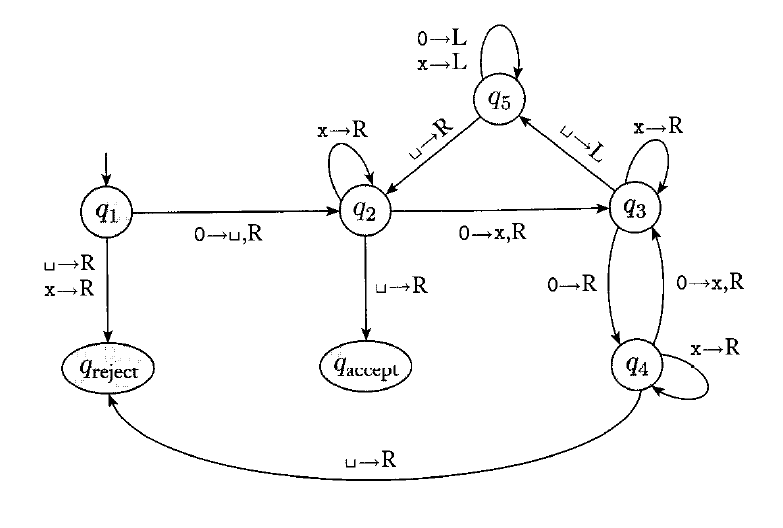
\includegraphics[width=0.7\linewidth]{images/mdt1}
	\end{center}
	Esempio di computazione di $M$ sull'input $0000$:
	\begin{center}
		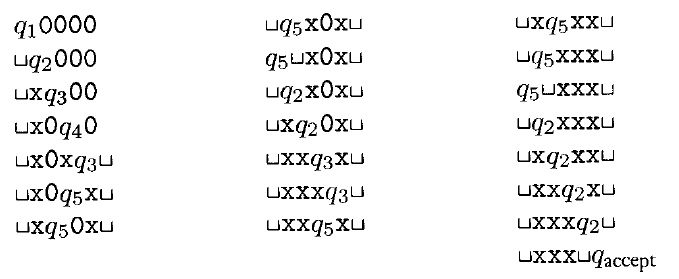
\includegraphics[width=0.5\linewidth]{images/mdt-run}
	\end{center}

	\pagebreak
	\subsection{Macchine di Turing multitape}
	Una macchina di Turing multi-tape è equivalente ad una macchina di Turing standard, con la differenza che sono disponibili $k$ nastri. Ogni nastro ha la propria testina per leggere e scrivere. Inizialmente i'input compare solo sul nastro $1$, mentre gli altri sono bianchi. La funzione di transizione cambia permettendo di leggere e scrivere su tutti i nastri simultaneamente. Formalmente
	\[
		\delta: Q \times \Gamma^k \to Q \times \Gamma^k \times \{ L,R \}^k
	\] 
	\begin{theorem*}
		Ogni macchina di Turing multitape può essere simulata con una macchina di Turing a nastro singolo.
	\end{theorem*}
	\begin{proof}
		Sia $M$ una MdT multitape e sia $S$ una MdT singletape. Definiamo che $M$ abbia $k$ nastri. Allora simuliamo in $S$ i $k$ nastri di $M$, memorizzando tutte le informazioni nell'unico nastro disponibile. Utilizziamo un nuovo simbolo $\sharp$ per delimitare il contenuto di un nastro dall'altro. Oltre a mantenere il contenuto di tutti i nastri, dobbiamo anche tener traccia della posizione della testina in ogni nastro (nastro virtuale dal momento che ne esiste solo uno). Per fare ciò marcheremo con un punto $\bullet$ il simbolo nel nastro che corrisponde alla posizione della testina su quel nastro.
		\begin{center}
			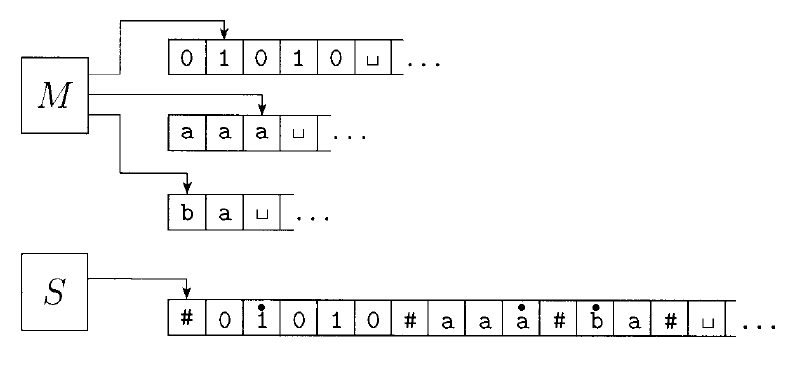
\includegraphics[width=0.7\linewidth]{images/mdt-multitape}
		\end{center}
		Per rappresentare una MdT con $k=3$ nastri con una MdT a nastro singolo dobbiamo:\\\\
		$S =$ input su $w_1,\dots,w_n$
		\begin{itemize}
			\item Porta il nastro di $S$ nella forma $\underbracket{\sharp\overset{\bullet}{w_1}w_2\dots w_n\sharp\overset{\bullet}{\text{\textvisiblespace}}\sharp\overset{\bullet}{\text{\textvisiblespace}}\sharp\dots\sharp}_{\text{$k$ pezzi}}$
			\item Scorri il nastro dal primo $\sharp$ all'ultimo $\sharp$ per determinare il contenuto delle testine
			\item Fai una seconda passata del nastro aggiornandolo
			\item Se $S$ muove una testina a destra di $\sharp$ allora rimpiazza $\sharp$ con \textvisiblespace\space e fai uno shift a destra di tutto	
		\end{itemize}
	\end{proof}

	\end{document}